\section{深度学习与强化学习}

\subsection{深度学习}
\subsubsection{深度学习的基本概念}
\begin{note}
    深度学习提出的背景
    \begin{enumerate}
        \item 非结构化大数据的涌现
        
        \item 特征工程的瓶颈
        
        \begin{itemize}
            \item 良好的\textcolor{main1}{特征表达},对最终算法的性能起了关键作用,而且系统主要的计算和测试工作都耗在这一部分。但是实际中一般是靠\textcolor{main1}{人工提取特征}。
            \item 机器学习中,获得好的特征是识别成功的关键。
            \item 人工选取特征费时费力,需要启发式专业知识,很大程度上靠经验和运气。
        \end{itemize}
        \item 自动特征提取:生物视觉机理的启发
        \begin{itemize}
            \item 机器可以自动地学习特征
            \item 人工神经网络是分层的;输入层输入原始图像,第一个隐层的神经元从中提取低层特征,后面隐层的神经元在此基础上获得高层特征;输出层用来分类。
        \end{itemize}
        \item 传统神经网络的局限
        
        BP算法无法胜任深层网络的训练
        \begin{itemize}
            \item 反馈调整时,梯度越来越稀疏,误差校正信号越来越小,容易出现梯度弥散或梯度消失现象;
            \item 容易收敛到局部最优,由于采用随机值初始化,当初值远离最优区域时易导致这一情况;
            \item 待训练的参数较多,需要大量有标签数据来训练,容易出现过拟合,无法用于无标签数据。
            \begin{figure}[htbp]
                \centering
                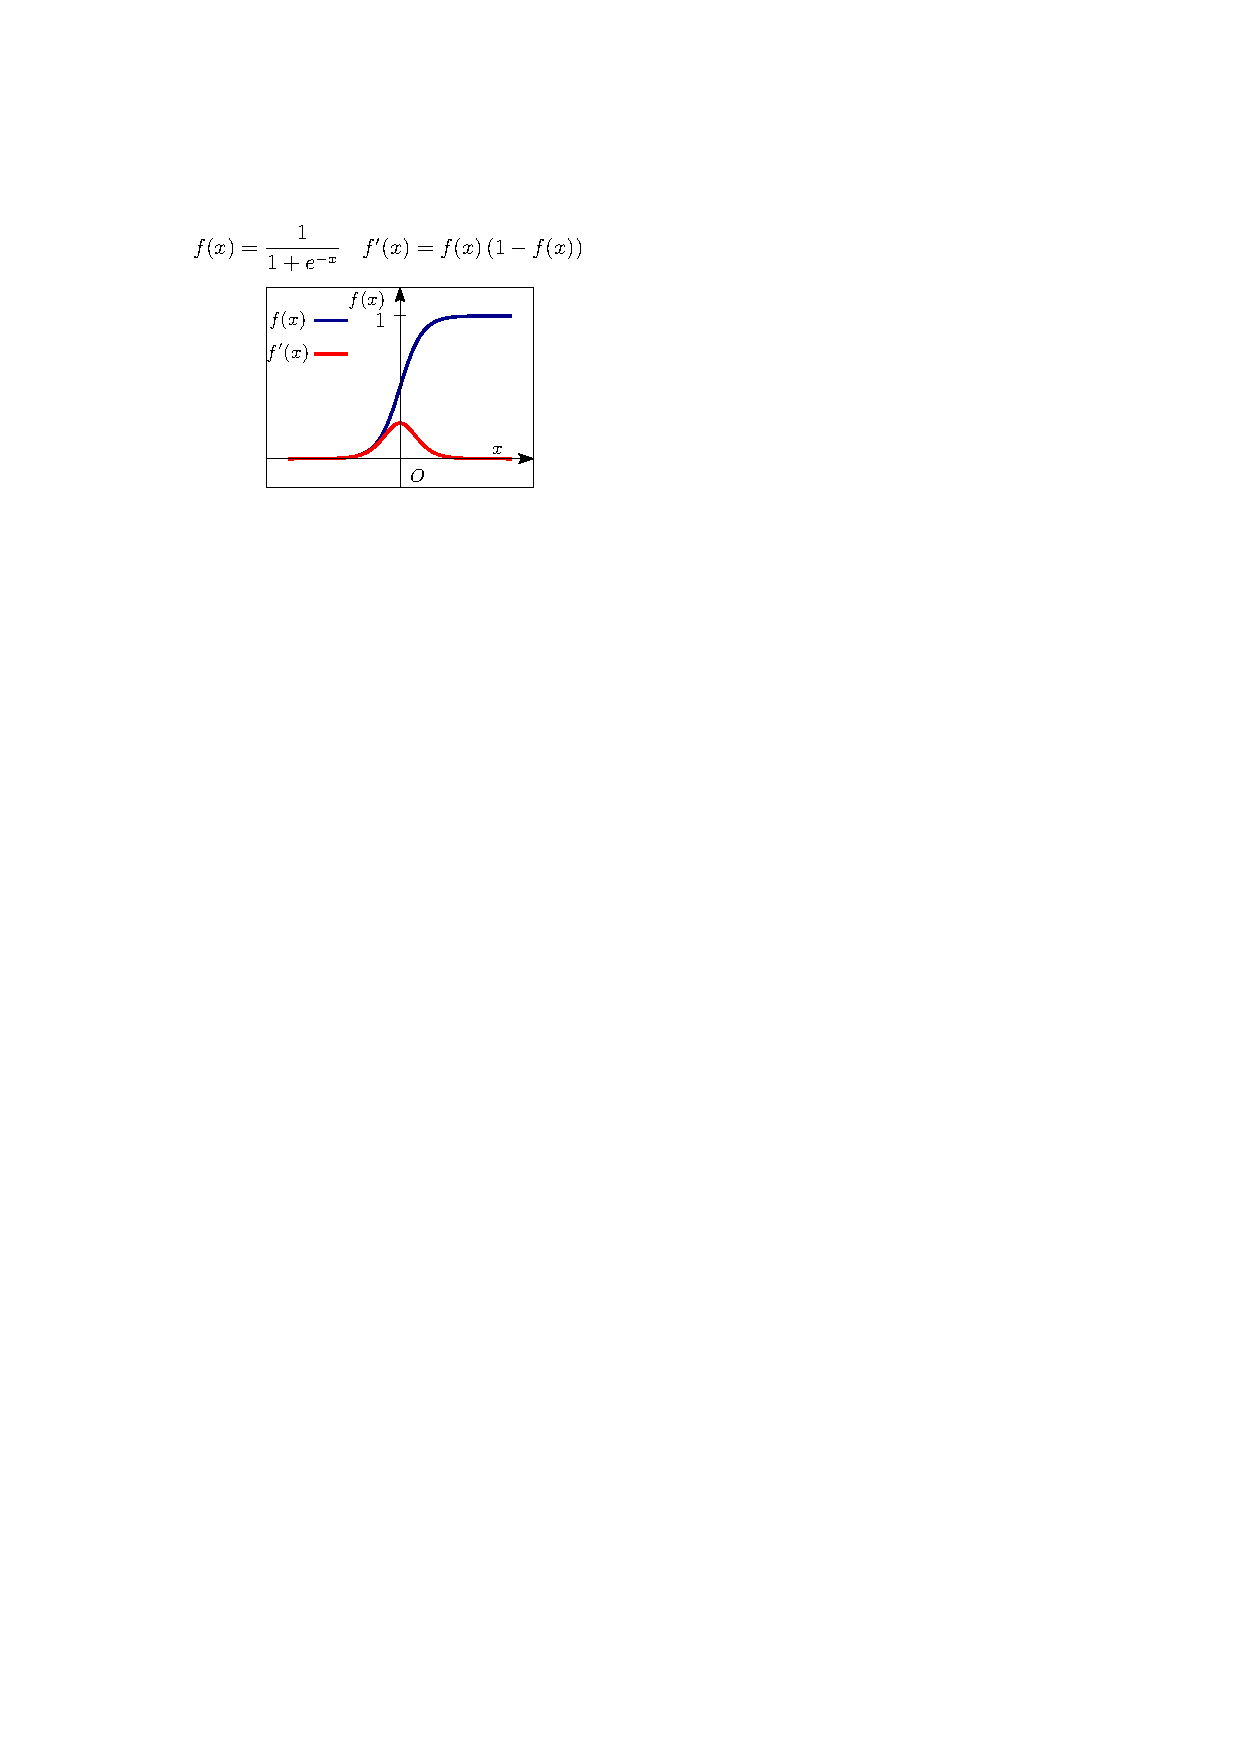
\includegraphics{image/梯度消失.pdf}
            \end{figure}
        \end{itemize}
    \end{enumerate}
\end{note}

\begin{definition}[深度学习的概念]
    深度学习是一种基于多层神经网络的机器学习方法,主要基于人工神经网络( Artificial Neural Network Network, ANN) 实现,是人工神经网络的“深度”版本,具有更强的数据表达能力。
\end{definition}
\begin{note}
    深度学习概念的分析
    \begin{itemize}
        \item 通过构建多隐层模型和海量训练数据(可为无标签数据),来学习更有用的特征,从而提升分类或预测的准确性。\textcolor{brown}{“深度模型”是手段,“特征学习”是目的。}
        \item 与浅层学习的区别
        
        强调了模型结构的深度,通常有5$\sim$10 个或更多的隐层。
        突出了特征学习的重要性,与人工提取特征的方法相比,利用大数据来学习特征,能够刻画数据的丰富内在信息。
        \item 深度学习网络的三要素
        \begin{itemize}
            \item 单元特性:多种函数可选
            \item 网络结构:多隐层的前向层次网络,主要为全连接
            \item 学习规则:逐层训练机制
        \end{itemize}
    \end{itemize}
\end{note}

\subsubsection{深度学习的训练过程}
\begin{note}
    深度学习的逐层训练方式
    \begin{enumerate}
        \item 第一步:采用自下而上的无监督学习
        \begin{itemize}
            \item 每次仅调整一层,每层采用wake sleep 算法进行调优。
            \item 这可以看作是一个特征学习的过程,是与传统神经网络区别最大的部分。
            \begin{itemize}
                \item wake阶段
                \begin{figure}[htbp]
                    \centering
                    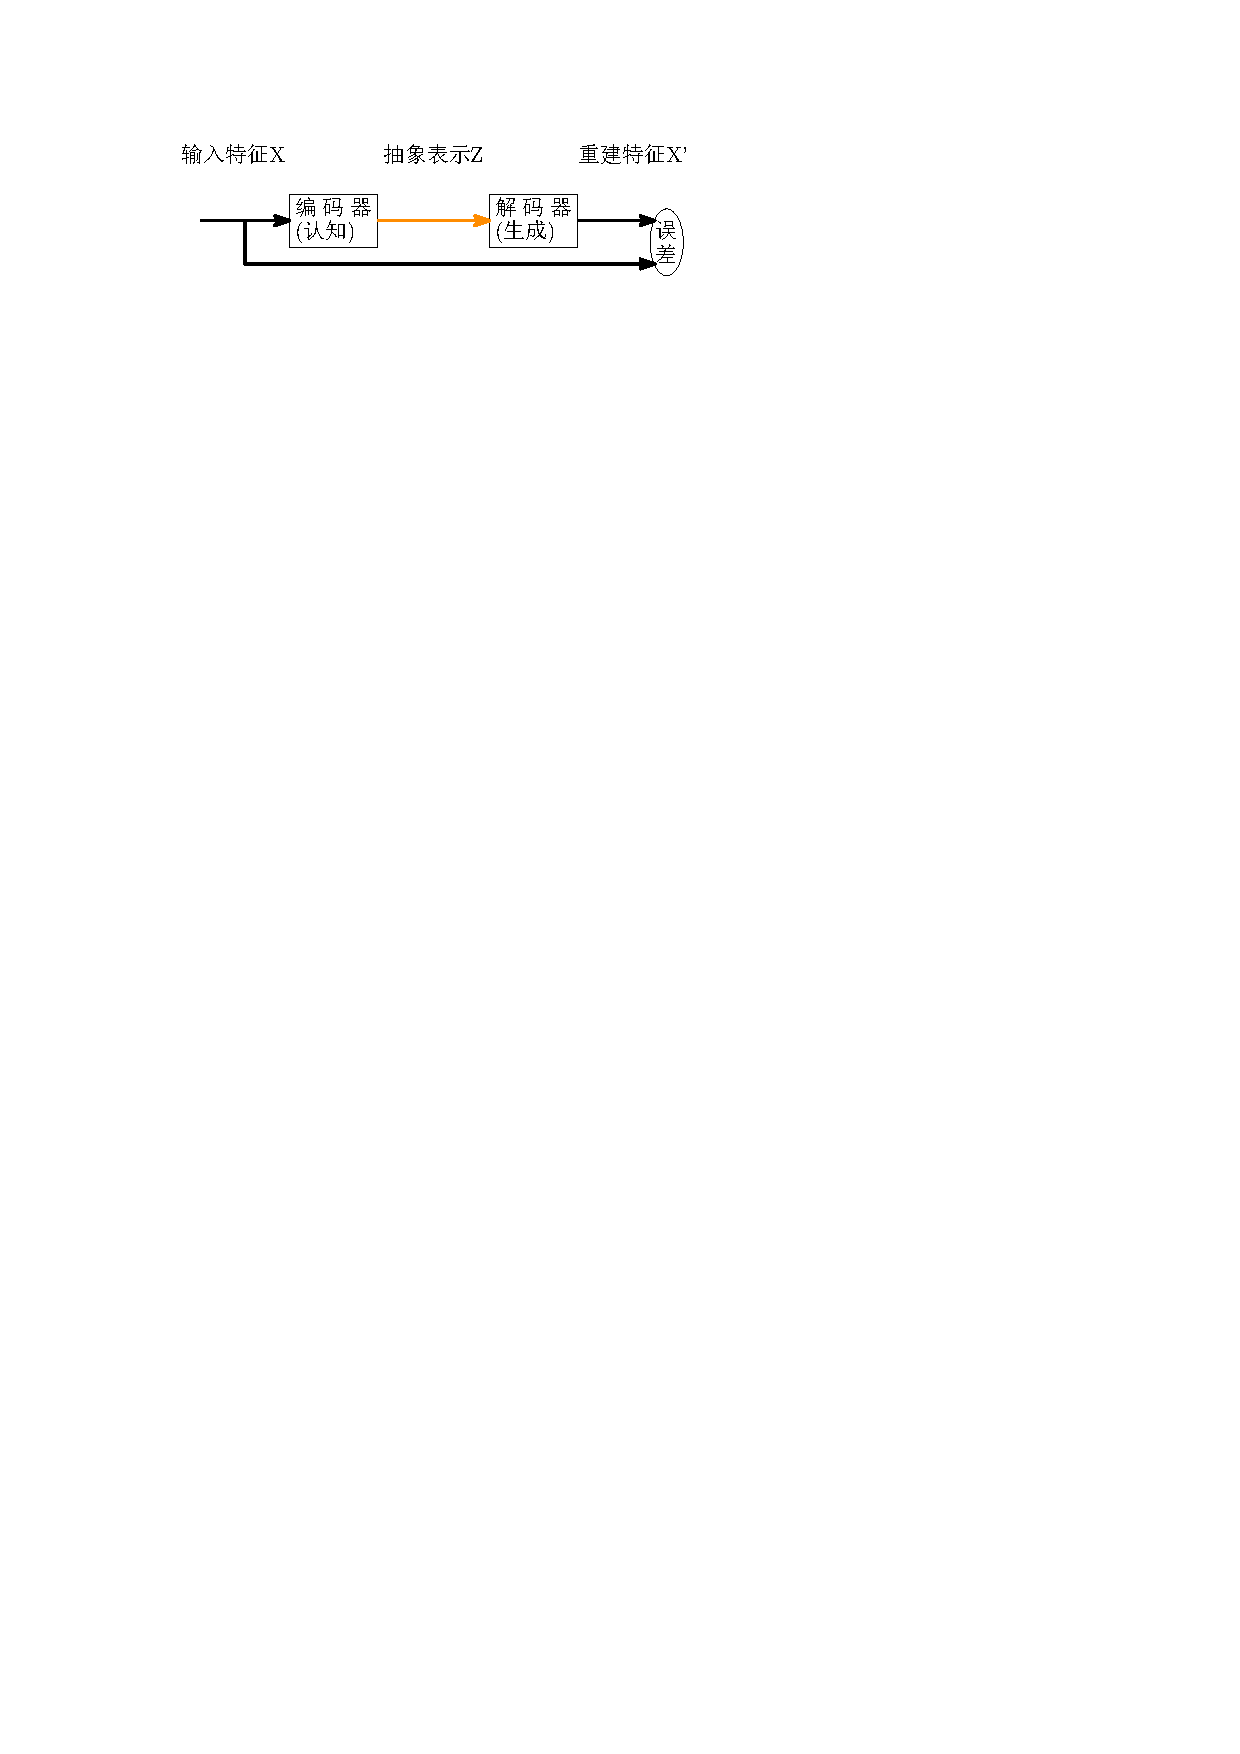
\includegraphics{image/wake.pdf}
                \end{figure}

                通过下层的输入特征X 和 编码器 上行的的认知权重产生每层的抽象表示Z,再通过当前(解码器)的生成权重产生重建信息X’,计算输入特征X 和重建信息X'的残差,使用梯度下降修改层间 (解码器)下行的生成(权重)。
                \item sleep阶段
                \begin{figure}[htbp]
                    \centering
                    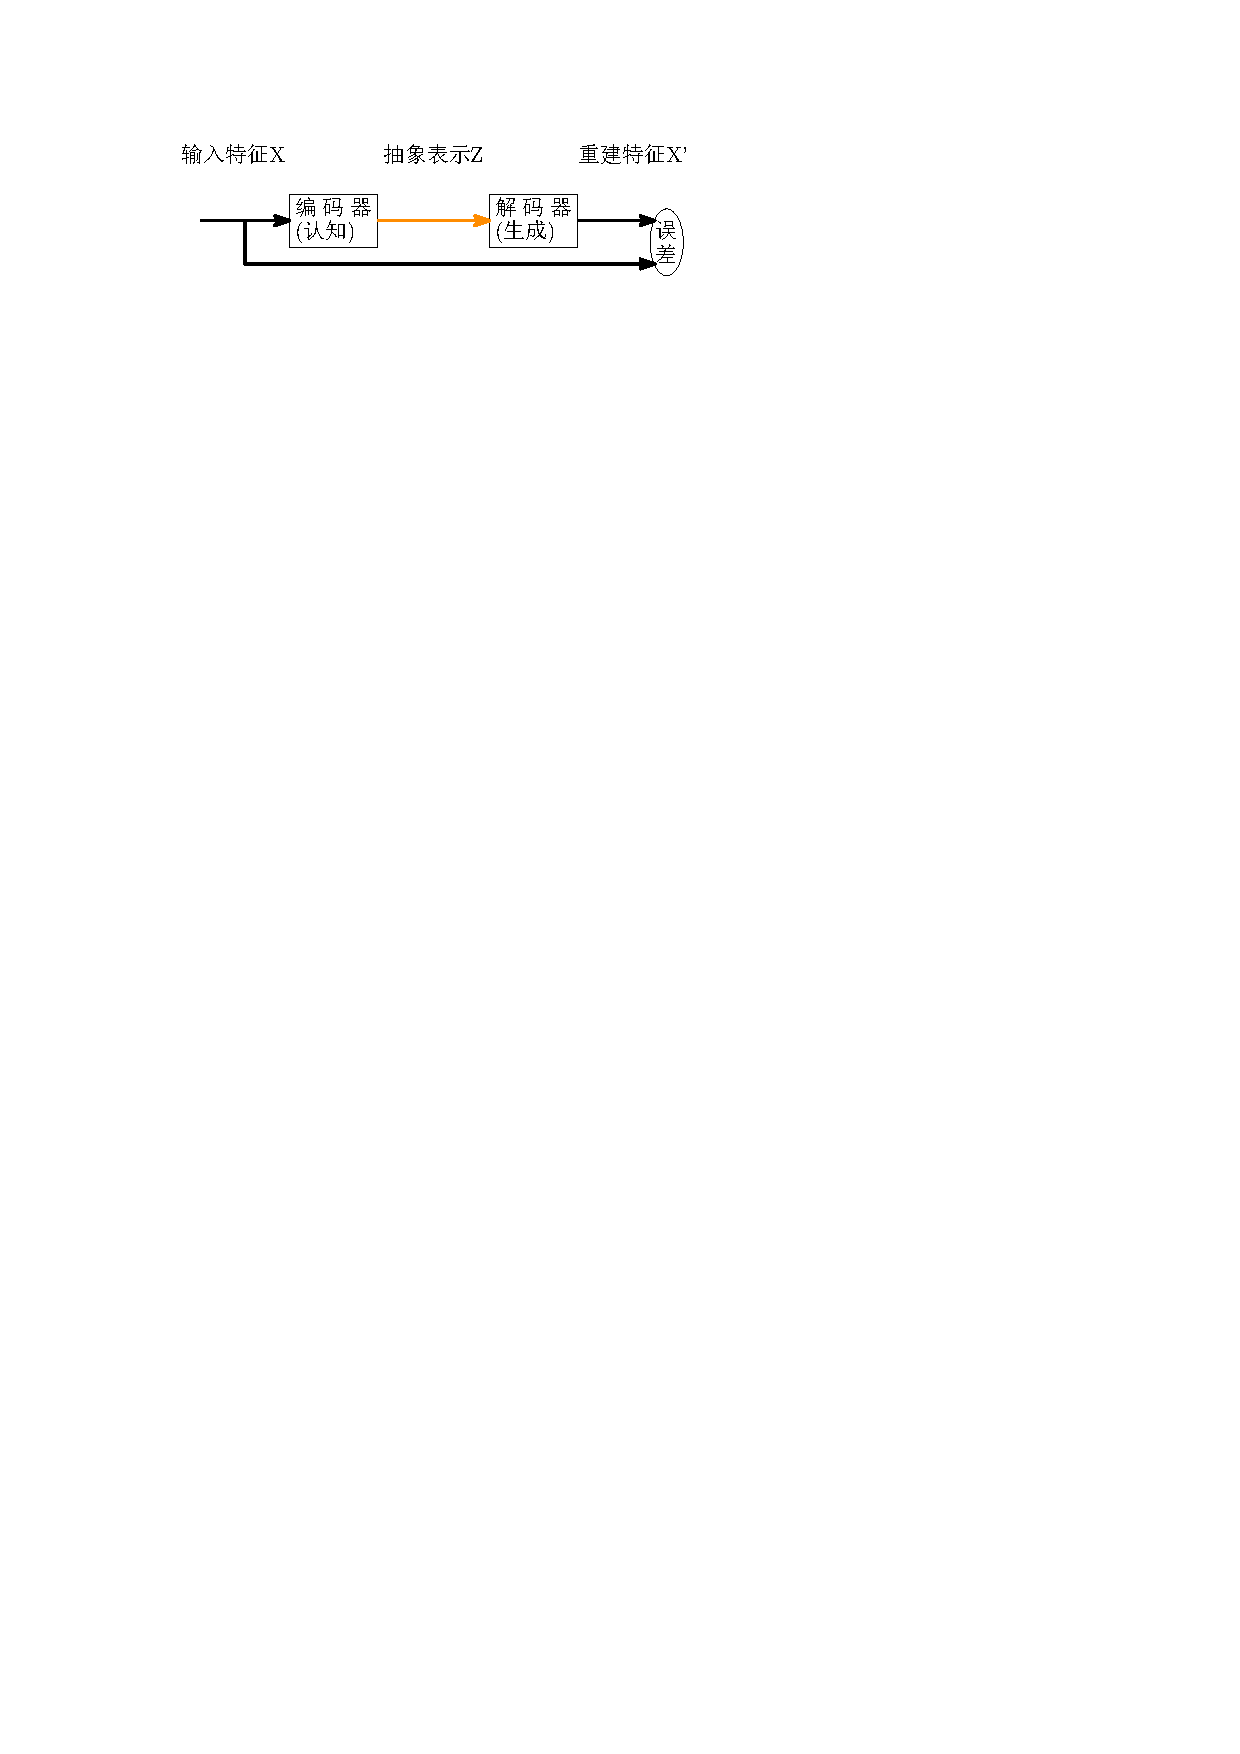
\includegraphics{image/wake.pdf}
                \end{figure}

                通过抽象表示Z 和 (解码器) 下行的生成权重,生成下层的特征X',再利用 (编码器) 上行的认知权重产生抽象表示Z' 。利用初始抽象表示Z 和新建的抽象表示Z' 的残差,利用梯度下降修改层间 (编码器) 上行的认知(权重)。
            \end{itemize}
        \end{itemize}
        \item 第二步:自顶向下的有监督学习
        
        在学习获得各层参数的基础上,在最顶的编码层添加一个分类器,通过带标签数据的有监督学习,利用梯度下降法去微调整个网络参数。
    \end{enumerate}
\end{note}
\begin{note}
    逐层训练方式的特点
    \begin{figure}[htbp]
        \centering
        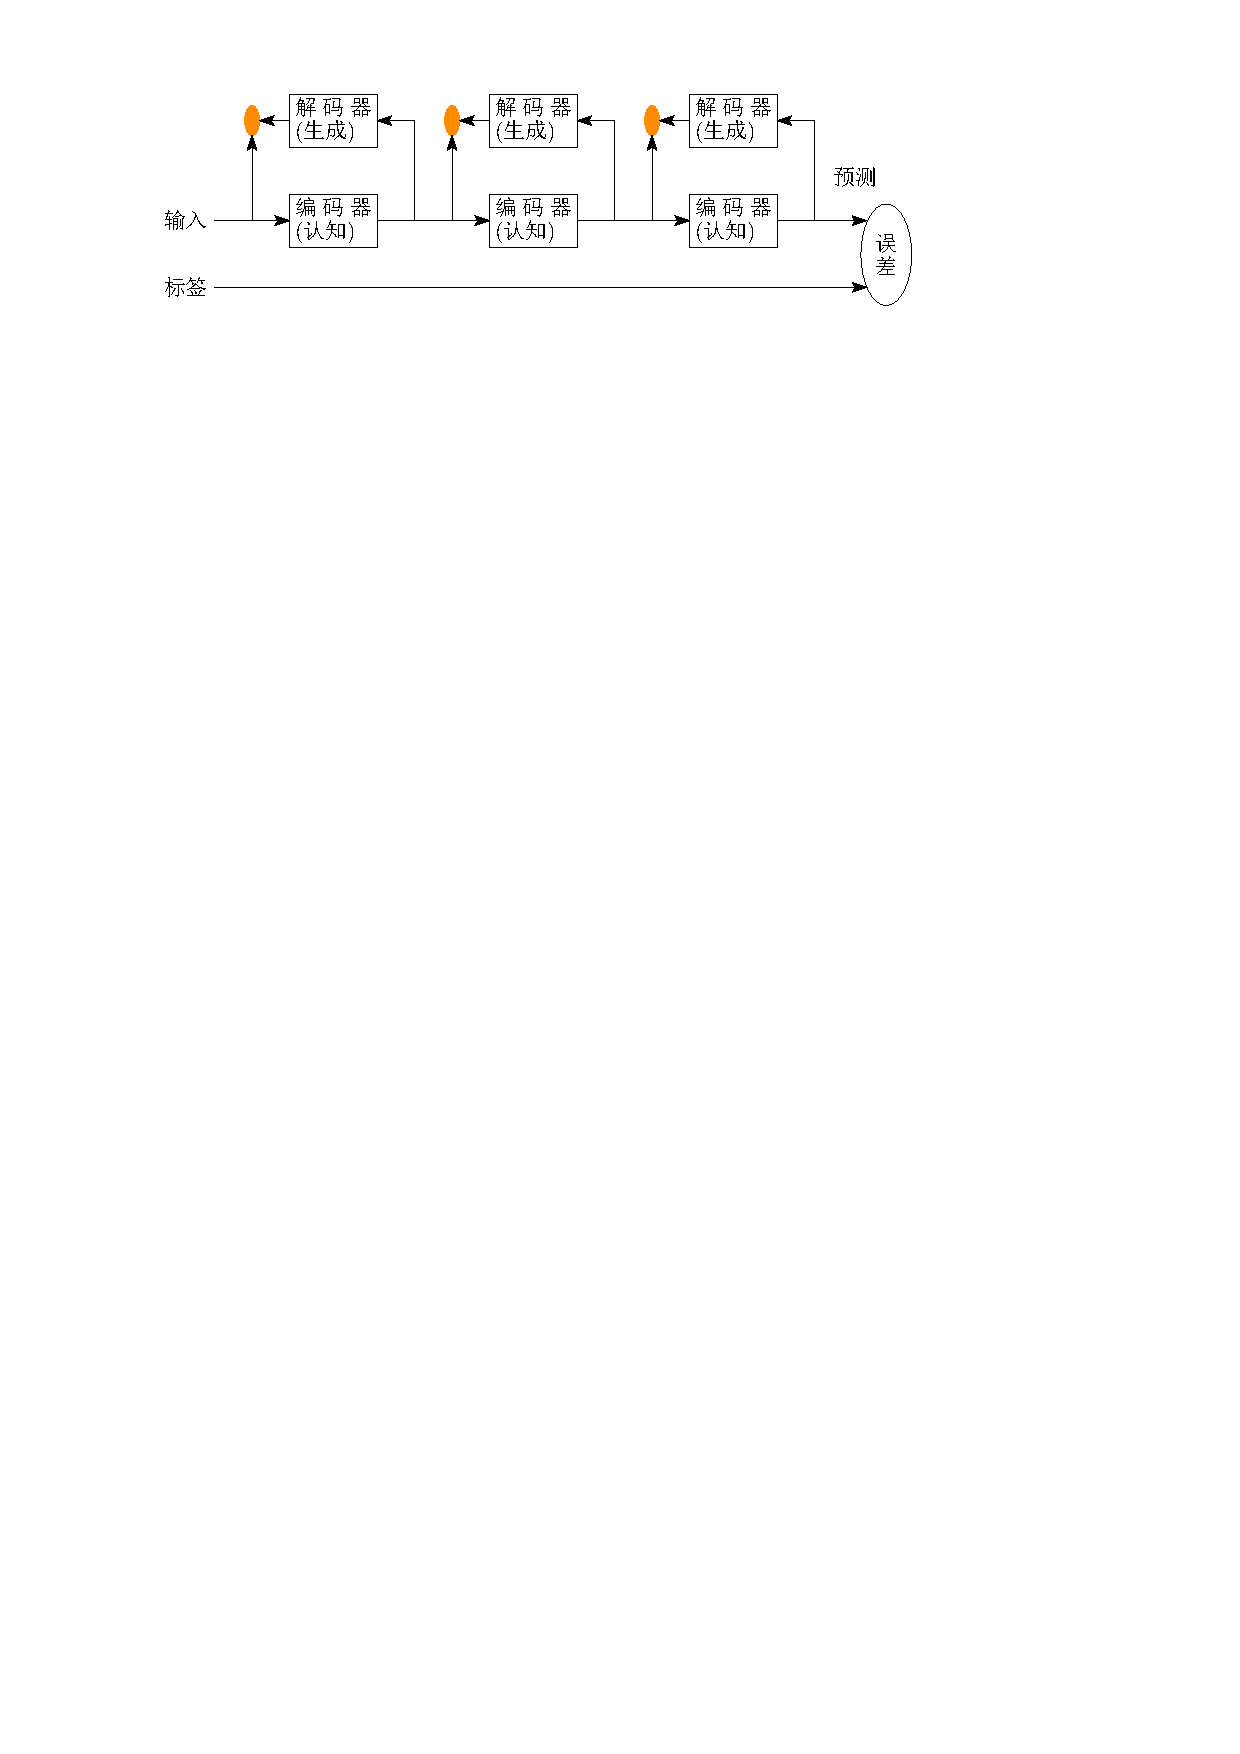
\includegraphics{image/逐层训练方式的特点.pdf}
    \end{figure}

    深度学习的第一步实质上是一个网络参数初始化过程。区别于传统神经网络的随机初始化,深度学习模型是通过无监督学习输入数据的结构得到的,因而这个初值更接近全局最优,能够取得更好的效果。
\end{note}
\begin{theorem}[通用逼近定理]
    通用逼近定理声明,包含至少一个隐层的多层前馈网络,只要其隐层神经元数量足够,能以任意精度逼近任意的连续函数。
\end{theorem}
\begin{note}
    深度学习的优势:通过学习深层非线性网络结构,实现复杂函数逼近,对输入数据进行分布式表示。
    \begin{itemize}
        \item 学习更加有效:深层网络含隐层数目较多而隐层的单元数量相对较少,如果浅层网络想达到同样的计算结果,需要\textcolor{main1}{指数级增长的单元数量}。使用更深层的模型可以减少表示函数所需的单元数,并减少泛化误差。
        \item 能够逐层提取特征:具有单隐层的前馈网络足以表示任何函数,但是该层\textcolor{main1}{可能过大而无法正确地学习和提取特征}。逐层加工处理是深度学习成功的关键因素。
        \item 通过学习一种深层非线性网络结构,实现复杂函数逼近,表征输入数据分布式表示;
        \item 能够自动提取特征,对于各层学习到的特征有更好的解释性;
        \item 能够更充分地利用无标签数据,不容易陷入局部最优;
        \item 结合大数据,不容易出现过拟合现象。
        \item 不需要人为特征提取,通过算法直接获取特征。在学习过程中不进行分模块或分阶段训练,直接优化任务的总体目标。中间过程不需要人为干预,使用起来更加方便。
    \end{itemize}
\end{note}

\begin{note}
    深度学习的局限性
    \begin{itemize}
        \item 主要体现在网络结构难设计、重复性差、结果不具可解释性、易受欺骗等,以及在小数据集上难以使用、黑箱模型、理论分析困难等。
    \end{itemize}
\end{note}
\begin{itemize}
    \item 典型有监督学习模型
    \begin{itemize}
        \item 卷积神经网络
        \item 循环神经网络
        \item 深度前馈神经网络
        \item 胶囊网络
    \end{itemize}
    \item 典型无监督学习模型
    \begin{itemize}
        \item 限制玻尔兹曼机
        \item 深度信念网络
        \item 生成对抗网络
        \item 自编码器
    \end{itemize}
\end{itemize}
\subsubsection{卷积神经网络}
CNN是一种带有卷积结构的深度神经网络,通常至少有两个可训练的卷积层(包括非线性作用函数)、两个池化层和一个全连接层,一共至少5个隐含层。
\begin{note}
    卷积神经网络主要执行四个操作:
    \begin{itemize}
        \item 卷积
        \item 非线性(ReLU)
        \item 池化或下采样
        \item 分类( 全连接层)
    \end{itemize}
\end{note}
\begin{note}
    卷积层
    \[
        S(m,n) = (\boldsymbol{I}*\boldsymbol{K})(m,n) = \sum\sum \boldsymbol{I}(m+i,n+j)\boldsymbol{K}(i,j)
    \]
    \begin{figure}[htbp]
        \centering
        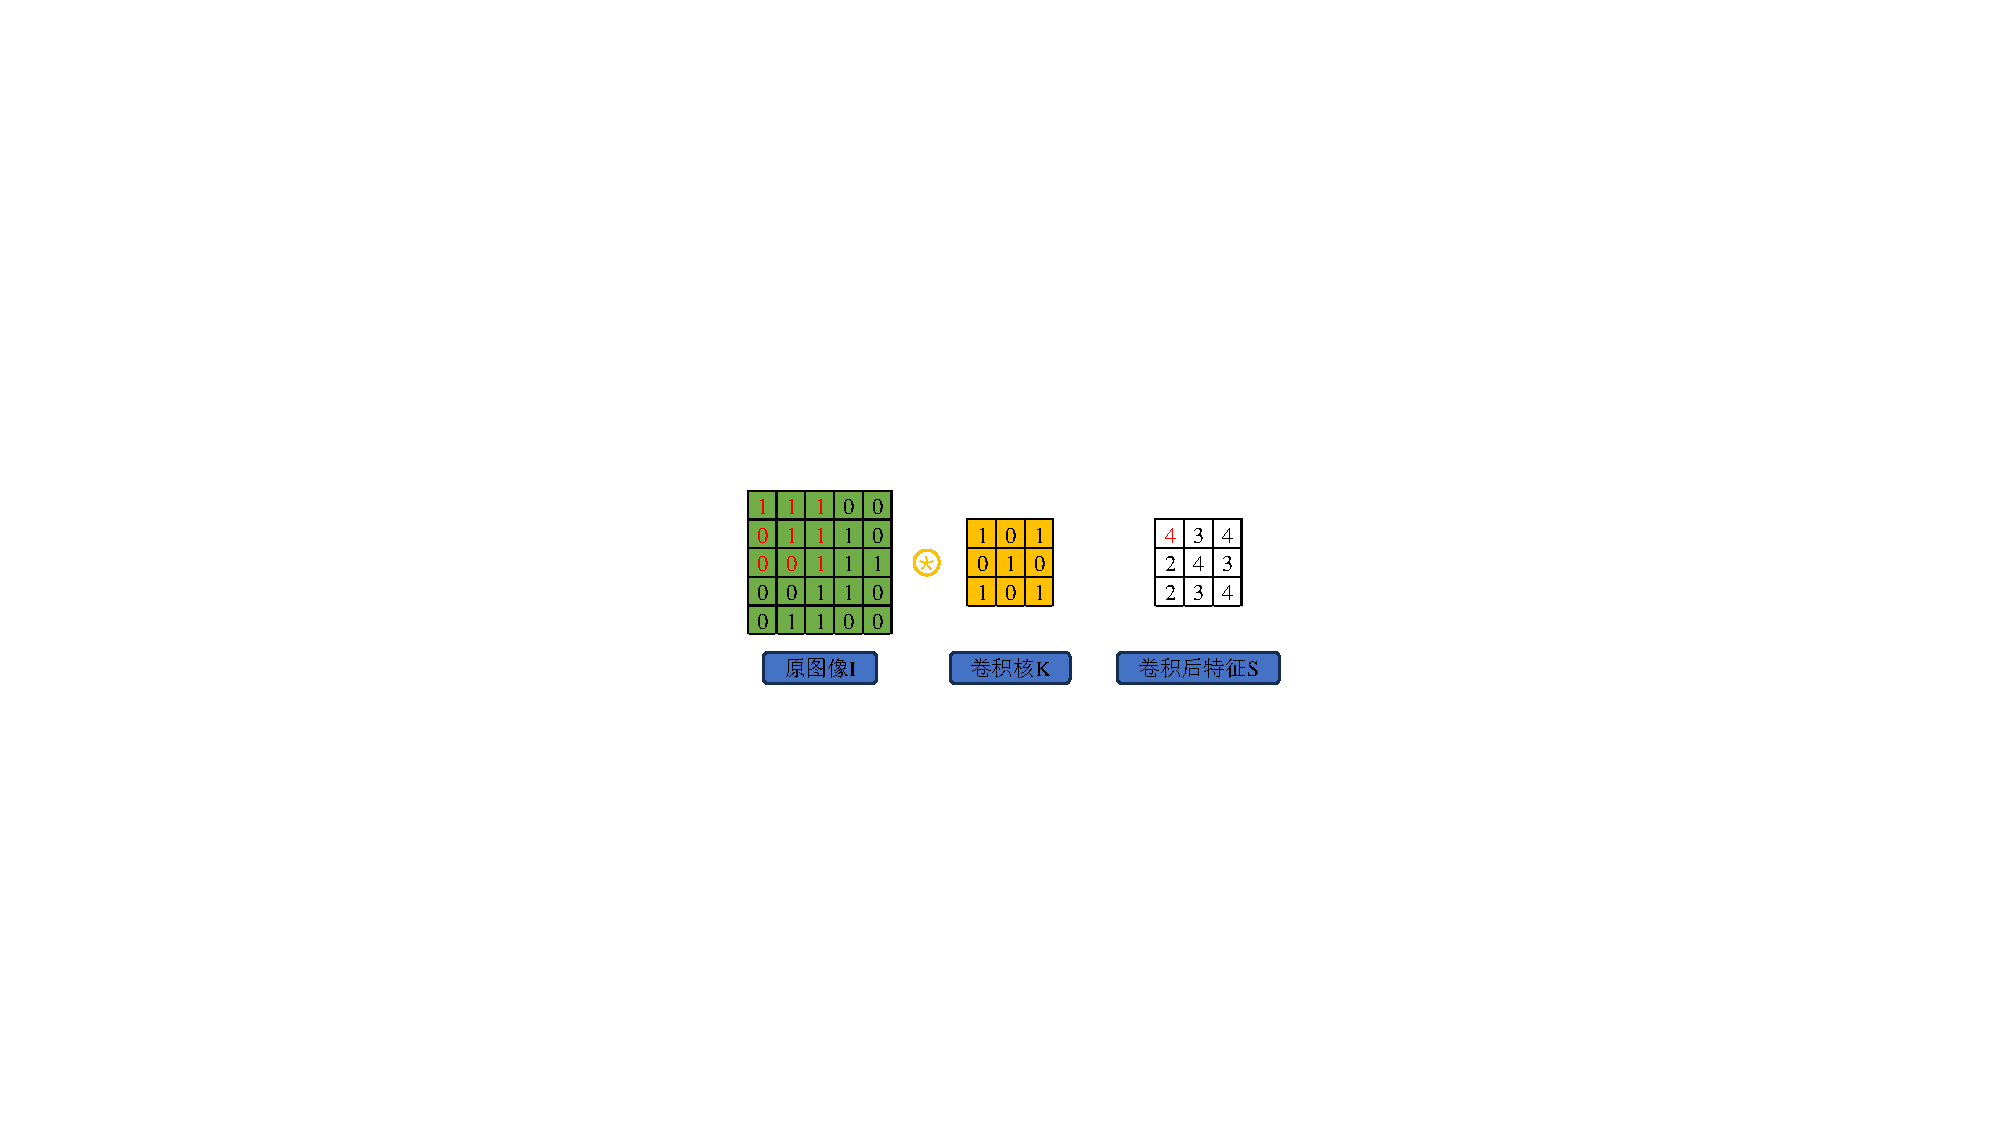
\includegraphics{image/卷积层.pdf}
    \end{figure}
\end{note}
\begin{note}
    池化层
    \begin{itemize}
        \item 池化层通常紧接着在卷积层之后使用,简化从卷积层输出的信息。
        \item 使用 “压缩”方法,通过一个下采样的过程,来减小图像的规模。
        \item 由于卷积得到的特征图中含有对于识别物体不必要的冗余信息,而通过下采样可以去除这些冗余信息,所以通常不会影响识别结果。
        \item 池化降低了每个特征映射的维度,但是保留了最重要的信息。
        \item 池化有多种形式:最大、平均、求和等。最大池化效果最好。
    \end{itemize}
    \begin{figure}[htbp]
        \centering
        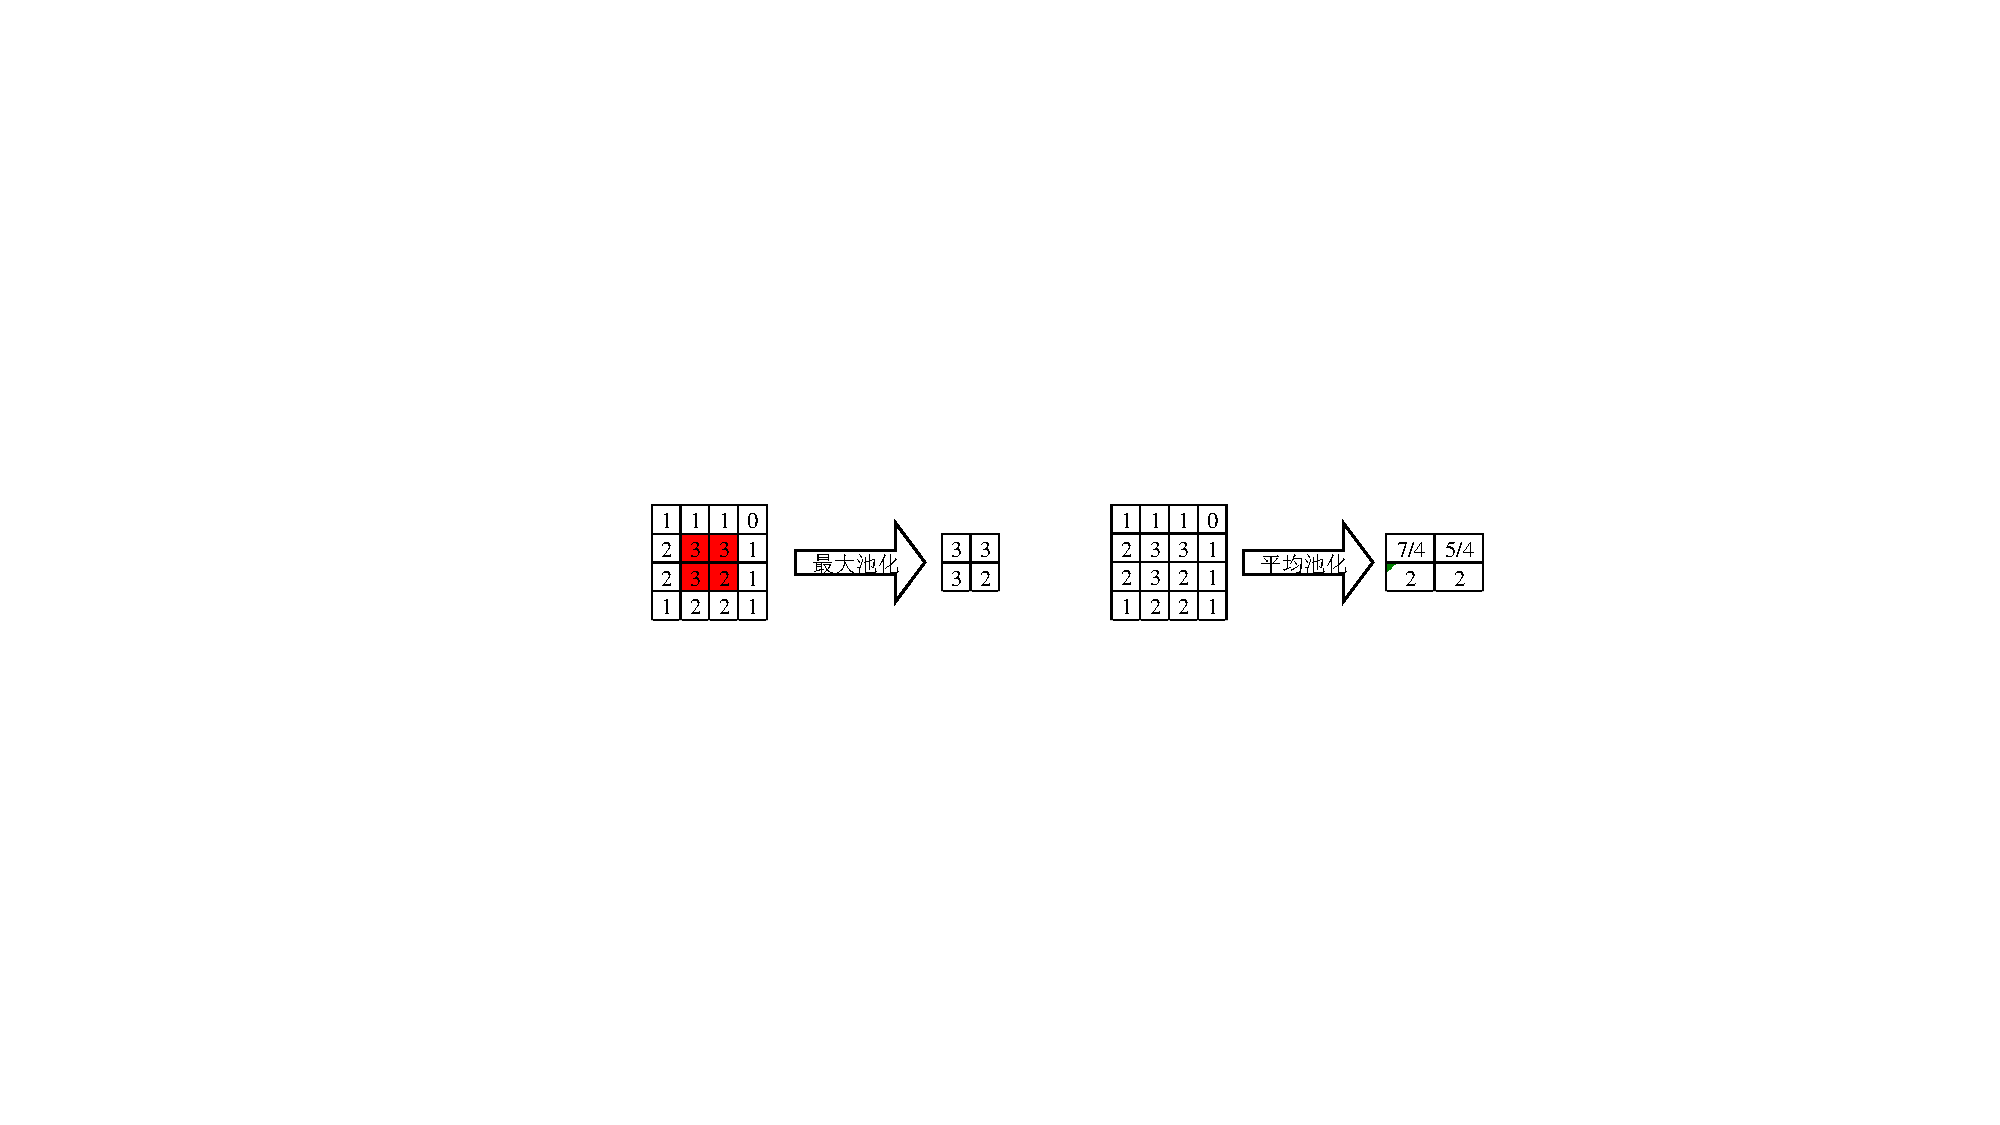
\includegraphics{image/池化.pdf}
    \end{figure}
    \textcolor{main1}{池化层的功能}
    \begin{itemize}
        \item 减少网络中待计算的参数数量,从而遏制过拟合
        \item 增强网络对输入图像中小变形、扭曲、平移的鲁棒性
        \item 帮助获得不因尺寸而改变的等效图片表征。
    \end{itemize}
\end{note}
\begin{note}
    非线性激励层
    \begin{itemize}
        \item 可用于卷积层和池化层之后,也可用于两层之间。
        \item 它是深度网络非线性的主要来源。
    \end{itemize}
    \begin{figure}[htbp]
        \centering
        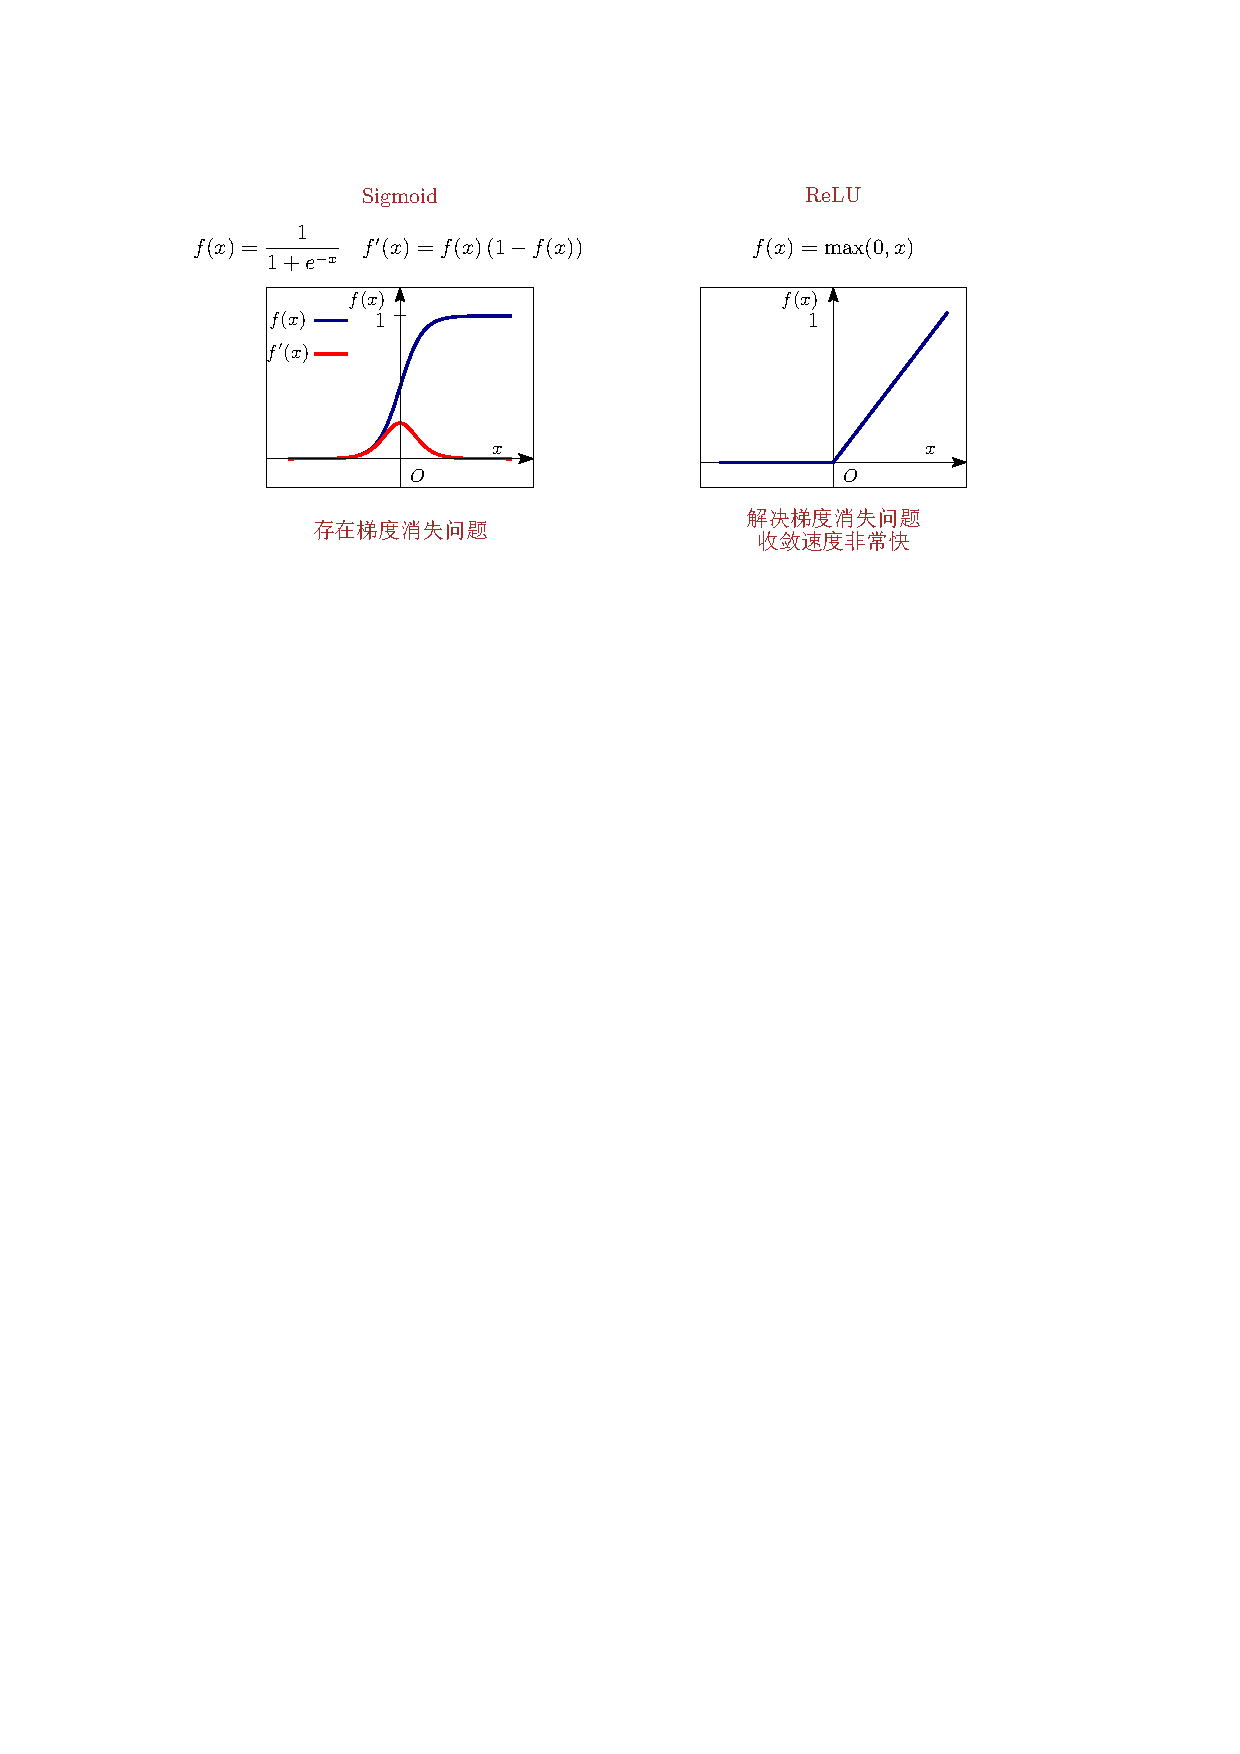
\includegraphics{image/非线性激励层.pdf}
    \end{figure}
\end{note}
\begin{note}
    全连接层和输出层
    \begin{itemize}
        \item 上层和下层的每个神经元之间都是相互连接的。
        \item 卷积层和池化层的输出代表了输入图像的高级特征,全连接层的目的是利用这些特征进行分类。
        \item 计算样本属于每类的概率作为输出。
        \item 输出层使用单极性Sigmoid函数或归一化指数函数(Softmax 函数)计算样本属于每类的概率,输出分类概率或标签。
    \end{itemize}
\end{note}
\begin{example}
    相对于全连接网络,卷积神经网络需要训练的参数规模大大减小,得益于下列哪些操作?
    \begin{enumerate}[A]
        \item \textcolor{main1}{卷积}
        \item \textcolor{main1}{池化}
        \item 非线性作用函数
        \item 全连接
    \end{enumerate}
\end{example}
\begin{note}
    常用的卷积网络整体结构
    \begin{figure}[htbp]
        \centering
        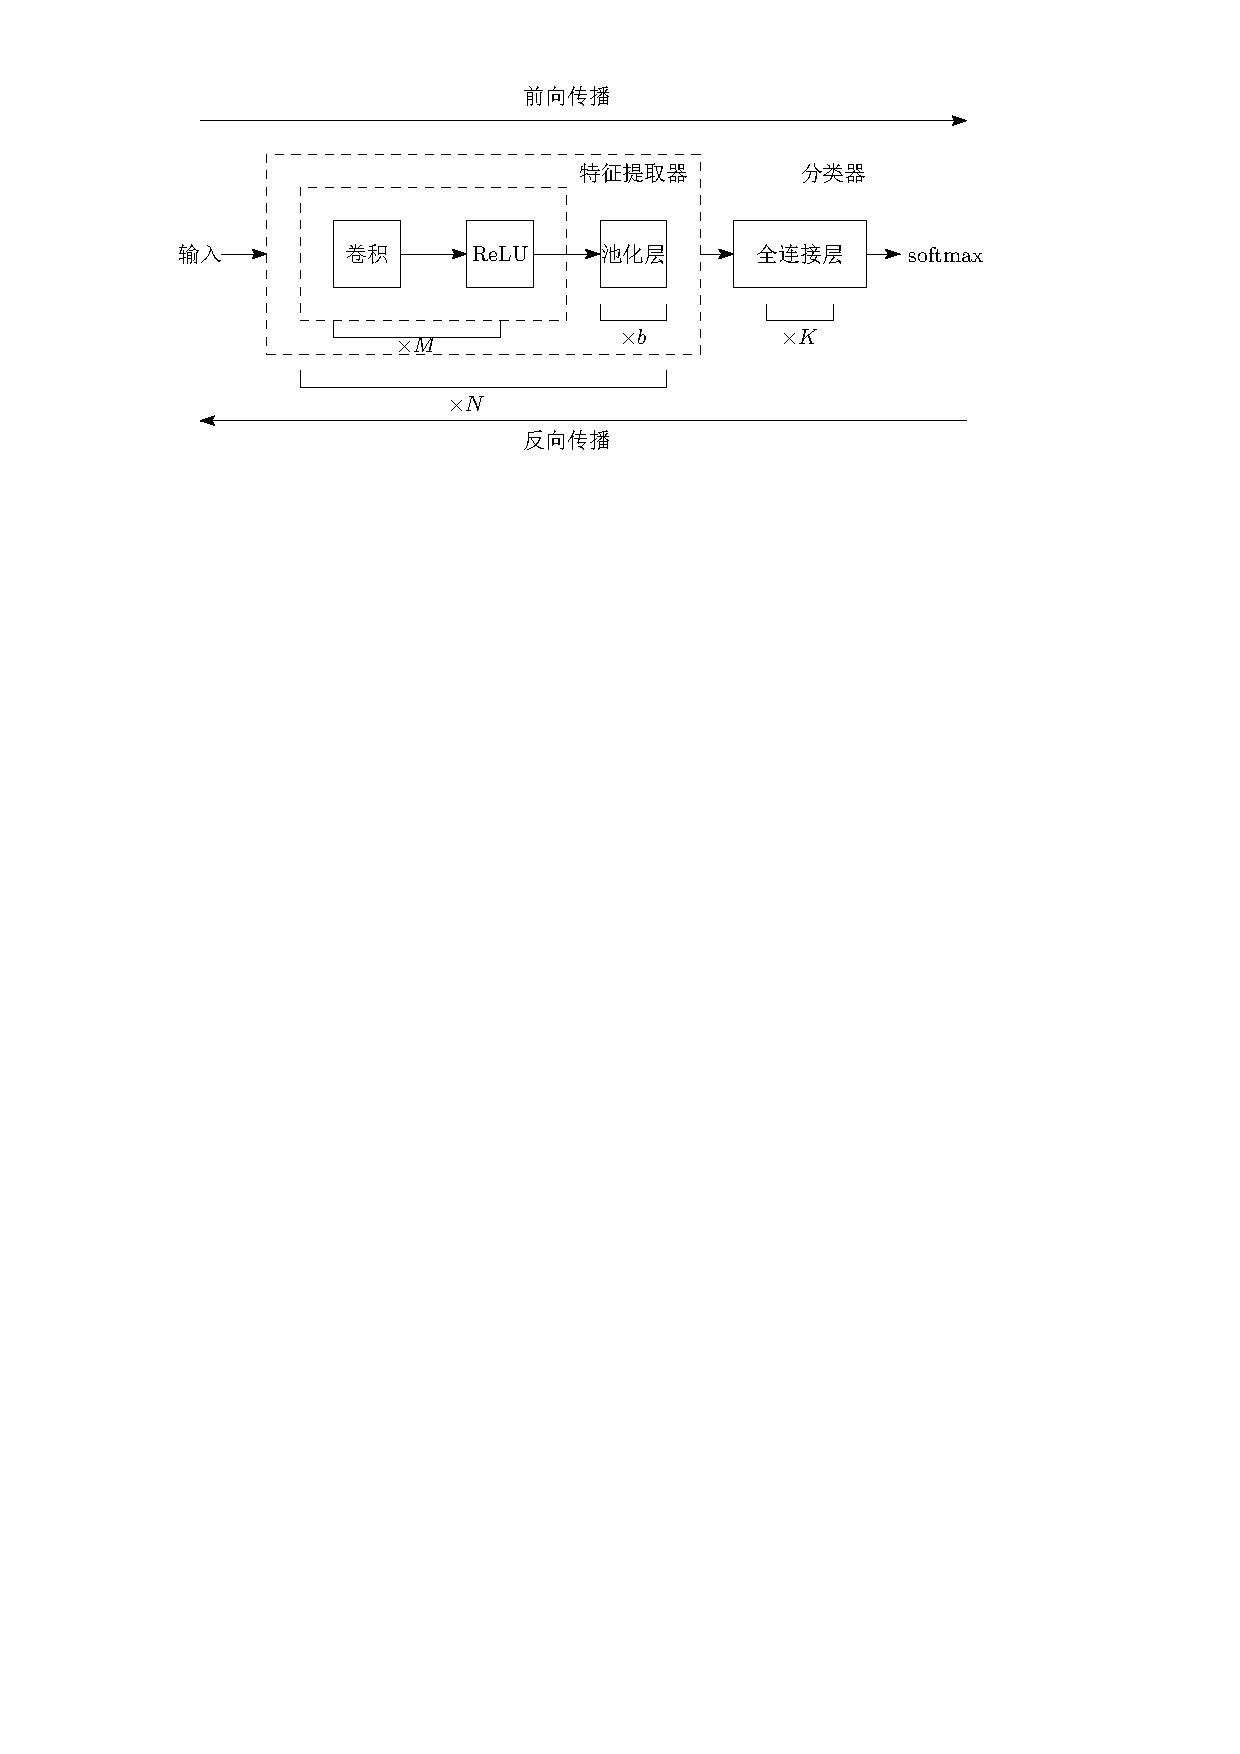
\includegraphics{image/CNN结构.pdf}
    \end{figure}
    \begin{itemize}
        \item 一个卷积块包括$M$个卷积层和 $b$ 个池化层( $M$ 通常设置为      $2\sim 5$, $b$ 为 0 或 1 )
        \item 一个卷积网络可以堆叠$N$个连续的卷积块,然后在后面接着 $K$ 个全连接层( $N$ 的取值区间比较大,如 $1\sim 100$ 或更大,K 一般为$0\sim 2$)
    \end{itemize}
\end{note}
\begin{example}
    卷积神经网络中需要学习的参数有:
    \begin{enumerate}[A]
        \item \textcolor{main1}{卷积核内的参数}
        \item 卷积核的数目
        \item 池化大小
        \item \textcolor{main1}{全连接权值}
    \end{enumerate}
\end{example}
\begin{note}
    现代深度学习的训练方法
    \begin{itemize}
        \item 避免欠拟合的方法
        \begin{itemize}
            \item 增加训练次数
            \item 改变网络结构,如增加网络的深度和每一个隐藏层的神经元个数
            \item 调整学习率
        \end{itemize}
        \item 避免过拟合的方法
        \begin{itemize}
            \item 数据增强(Data Augmentation)
            
            旋转、缩放、翻转、加噪声
            \item 使用合适的模型:减少网络的层数、神经元个数
            \item 正则化
            
            通过约束权重的L1范数或者L2范数,对模型的复杂度进行惩罚,减小模型在训练数据集上的过拟合。

            \[
                \begin{array}{l}
                    E_1 = E+\frac{\lambda}{2}\sum\sum(\ ^{l}w_{ij})^2\\
                    \delta\ ^{l}w_{ij} = -\eta\left( \dfrac{\partial E}{\partial\ ^{l}w_{ij}}+\lambda\ ^{l}w_{ij} \right)
                \end{array}
            \]
            \item Dropout
            
            在深度网络学习的训练过程中,对于神经网络单元,按照一定的概率将其暂时从网络中丢弃。(\textcolor{red}{在网络测试时不丢弃神经元!})
            \item 限制训练时间;或者通过评估测试,提前终止训练
            
            在每次迭代时,把新学习到的模型在验证集上进行测试,并计算错误率。验证集上的错误率通常会先下降后上升,拐点处预示着开始过拟合,就停止迭代。
            \begin{figure}[htbp]
                \centering
                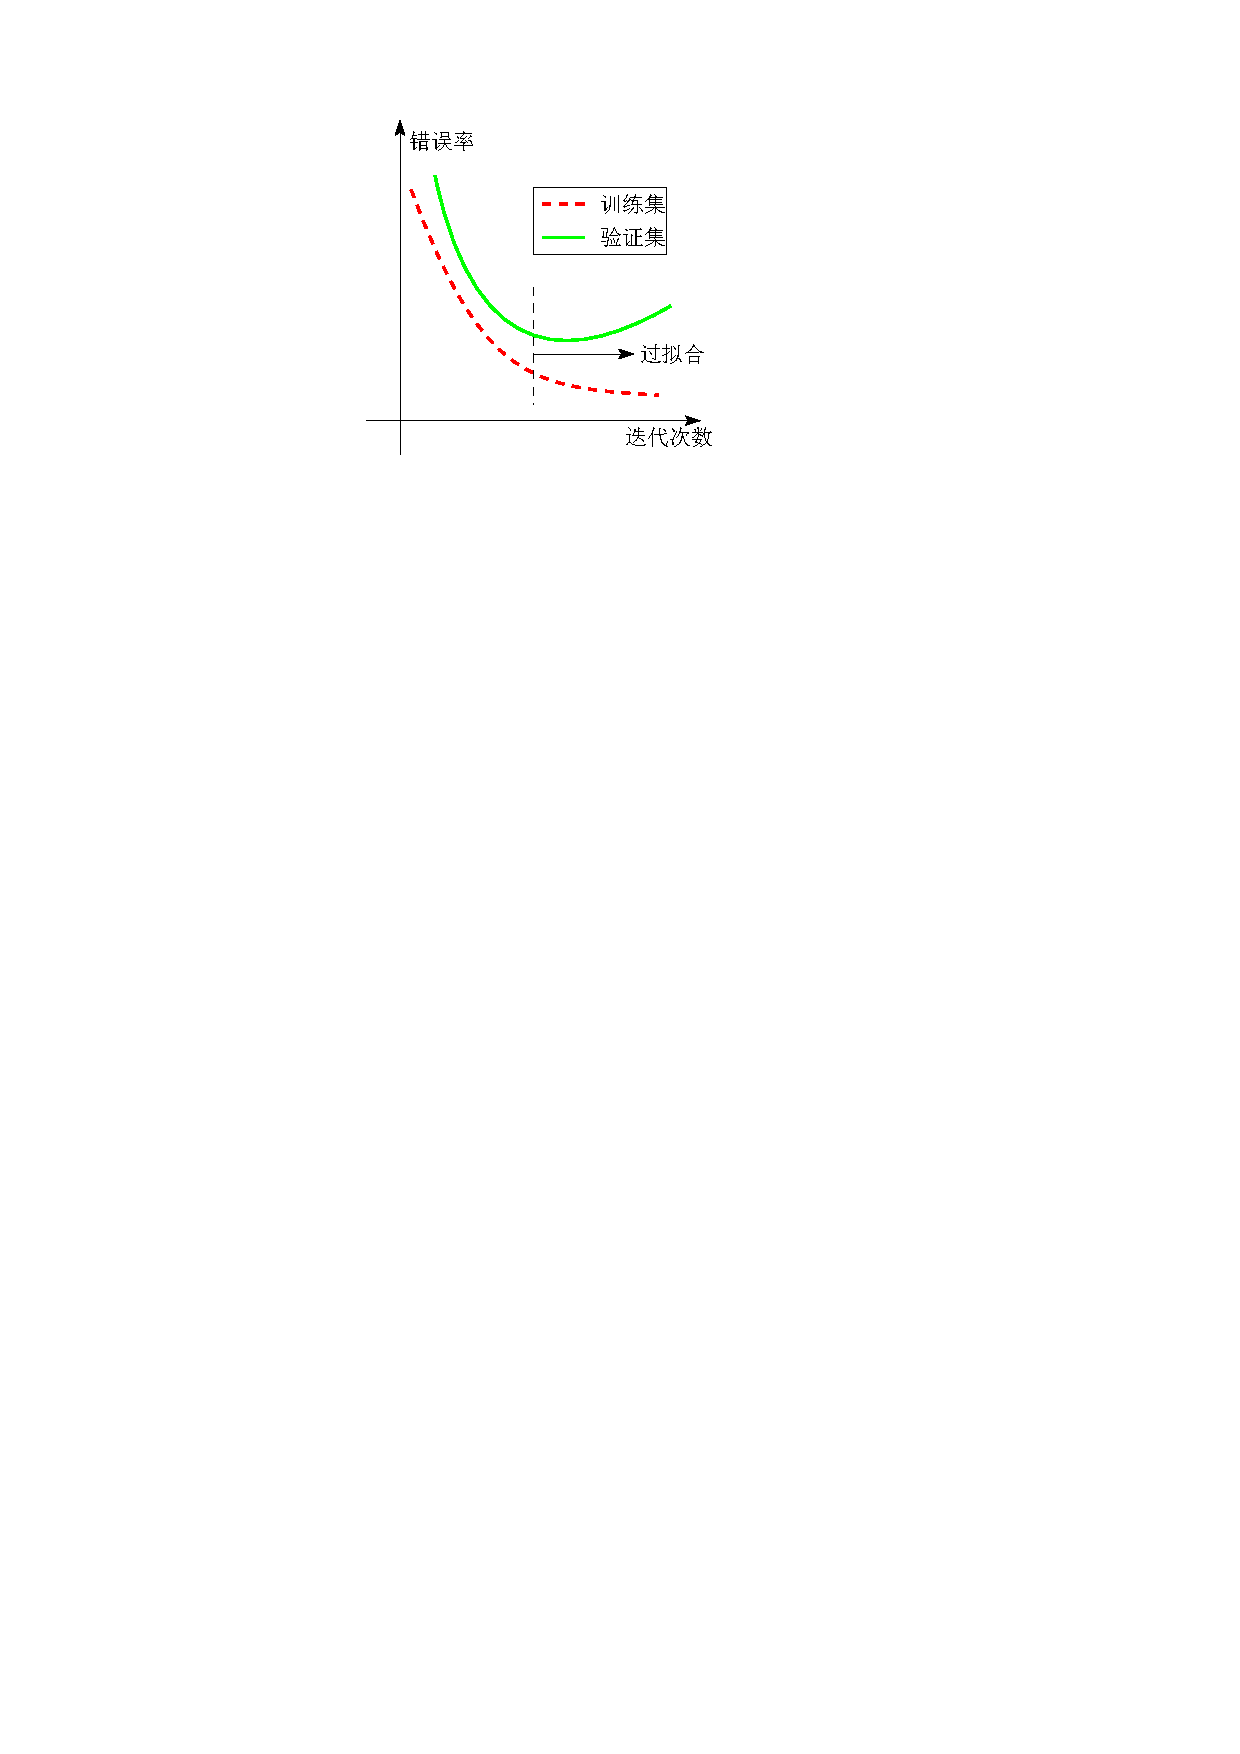
\includegraphics{image/提前停止.pdf}
            \end{figure}
        \end{itemize}
    \end{itemize}
\end{note}
\subsection{强化学习}
\subsubsection{强化学习基本概念}
\begin{definition}[强化学习]
    强化学习是一种从环境状态到动作映射的学习,目标是使动作从环境中获得的累积奖赏值最大。

    强化学习的生理基础:强化学习的最重要的反馈信号是多巴胺
    \begin{figure}[htbp]
        \centering
        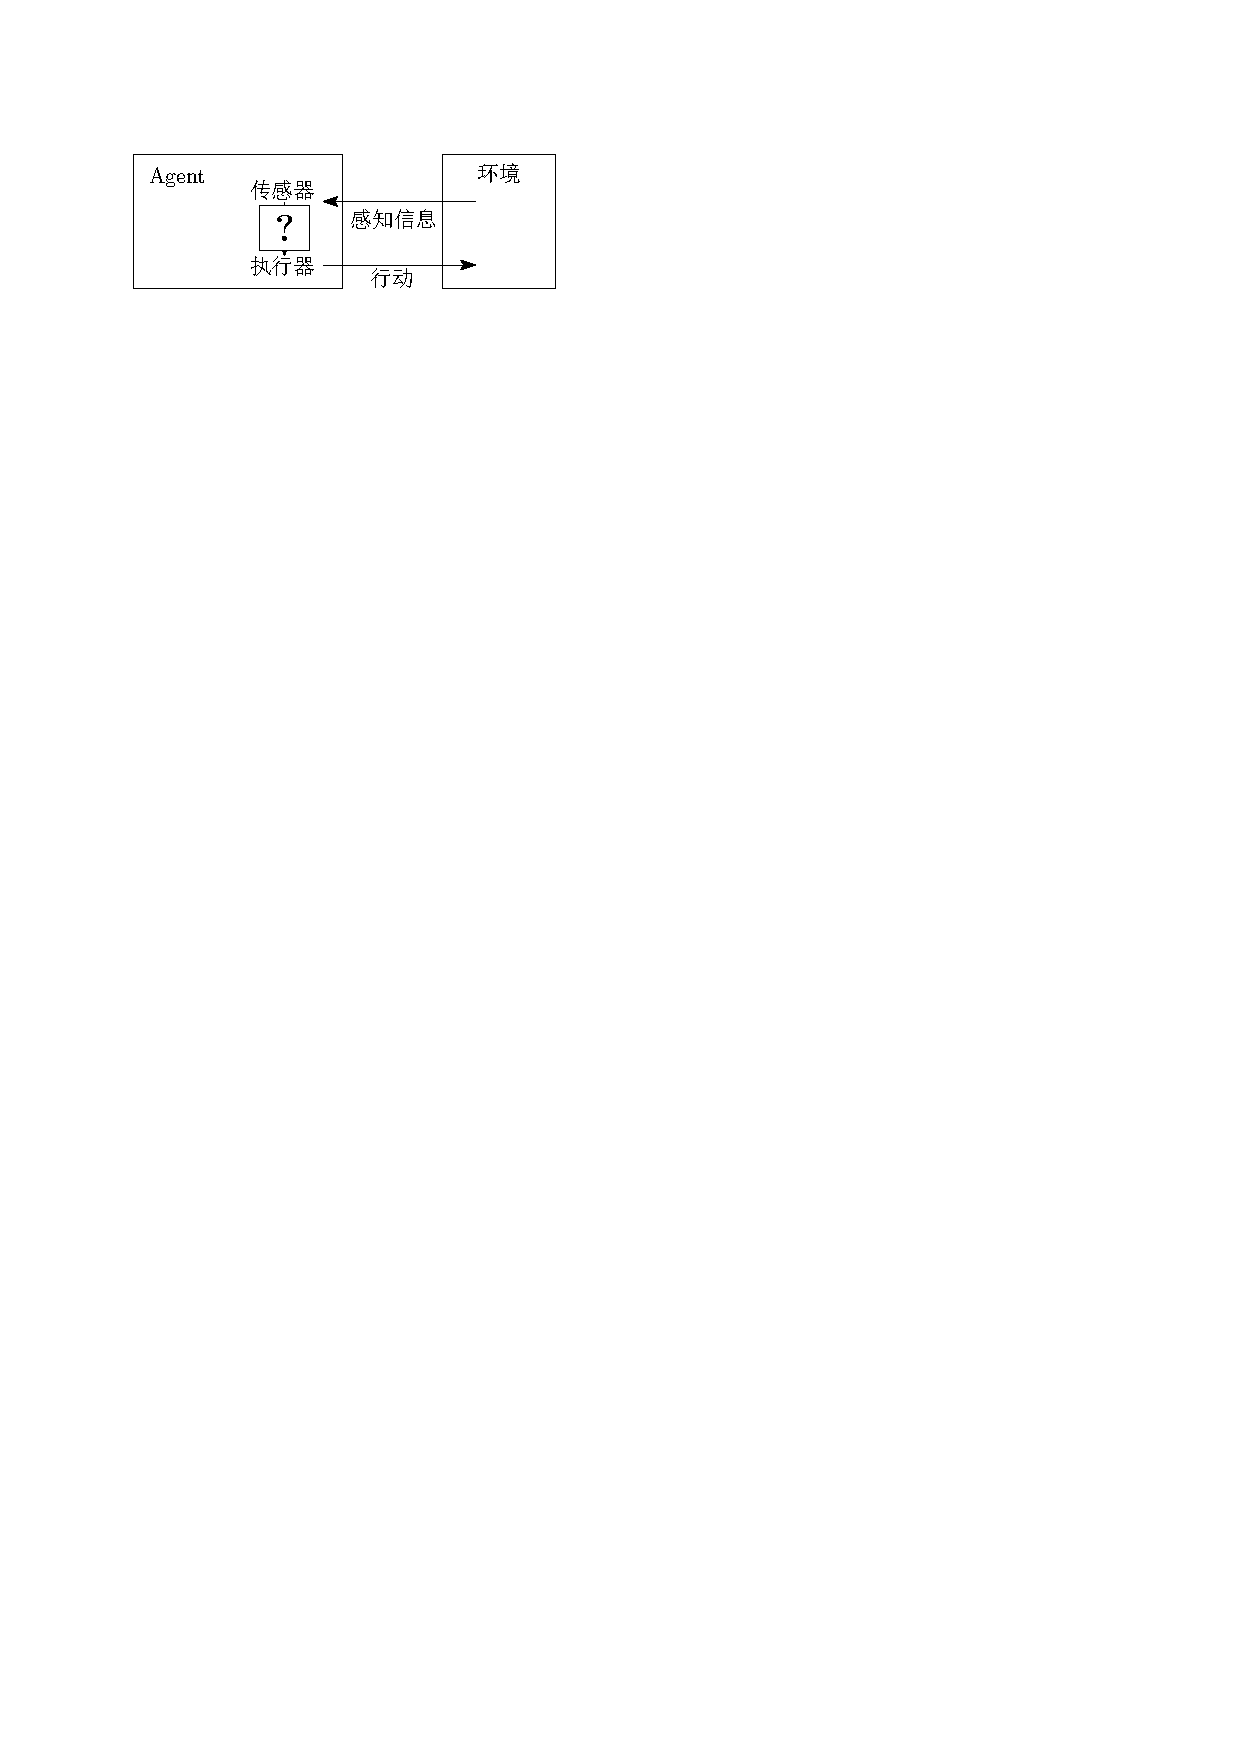
\includegraphics{image/Agent.pdf}
    \end{figure}
    基本思想
    \begin{itemize}
        \item Agent以奖励的形式得到环境的反馈;
        \item Agent学习如何更好行动以极大化累积奖励;
        \item 基于观察环境反馈的结果进行学习。
    \end{itemize}
\end{definition}
\begin{note}
    强化学习中的常用术语
    \begin{itemize}
        \item Agent:在环境中执行动作以获得奖励的某个实体
        \item 环境$(e)$:Agent 面对的场景
        \item 奖励$(r)$:Agent 执行特定动作或任务时获得的收益
        \item 状态$(s)$:状态是指环境返回的当前状态
        \item 策略$(\pi)$: Agent 根据当前状态决定下一步采取什么动作
        \item 价值$(V)$:将来累积总收益的期望值。
        \item 价值函数$V (s)$:用价值函数来对当前状态进行估价,进入现在这个状态,可以对Agent 后面的收益带来多大的影响。当这个价值函数大的时候,说明Agent 进入这个状态越有利。
        \item 环境模型: 模型表示了Agent 对这个环境的状态进行了理解。
        \item Q值或行动值$(Q(s,a))$:Q 值与价值非常相似,对(状态-动作)对进行评价。
    \end{itemize}
\end{note}
\begin{note}
    强化学习方法的分类:
    \begin{itemize}
        \item 基于使用策略与使用值函数,强化学习算法分为三类:
        \begin{itemize}
            \item 基于值函数的强化学习算法
            \item 基于策略的强化学习算法
            \item Actor Critic 算法
        \end{itemize}
        \item 基于是否使用模型,强化学习算法分为两类:
        \begin{itemize}
            \item 无模型算法(Model Free)
            \item 基于模型的强化学习算法(Model Based)
        \end{itemize}
    \end{itemize}
    \textcolor{red}{“模型”特指环境,即环境的动力学模型,与深度学习中的模型不同。}
\end{note}
\begin{example}
    强化学习的主要特点有那哪些?
    \begin{enumerate}[A]
        \item \textcolor{main1}{Agent需要通过探索环境来获取对环境的理解}
        \item \textcolor{main1}{Agent执行动作从环境里面获得奖励}
        \item \textcolor{main1}{在训练过程中,时间非常重要。因为Agent 得到的数据都是有时间关联的(sequential data),而不是独立同分布的}
        \item \textcolor{main1}{Agent的行为会影响它随后得到的数据}
    \end{enumerate}
\end{example}
\subsubsection{马尔科夫决策过程}
\begin{note}
    5个关键要素:
    \begin{itemize}
        \item $S$为有限的状态集
        \item $A$为有限的动作集
        \item $P$为状态转移概率
        \[
            P_{ss'}^{a} = P\left( S_{t+1}=s'|S_t = s,A_t = a \right)
        \]
        \item $R$为奖励函数
        \[
            R_{ss'}^{a} = E\left( R_{t+1}|S_t = s,A_t = a,S_{t+1} = s' \right)
        \]
    \end{itemize}
    Agent的目标是最大化回报值:($\gamma\in[0,1]$为折扣因子)
    \[
        G_t = R_{t+1}+\gamma R_{t+2}+\gamma^2R_{t+3}+\cdots
    \]
\end{note}
\begin{note}
    马尔科夫决策过程数学模型
    \begin{itemize}
        \item 在随机过程中,假设状态历史为$h_t = \left\{ s_0,\cdots,s_t \right\}$,马尔科夫性是指当前状态的下一个状态只取决于当前状态,
        \[
            \begin{array}{l}
                P\left( s_{t+1}|s_t \right) = P\left( s_{t+1}|h_{t} \right)\\
                P\left( s_{t+1}|s_t,a_t \right) = P\left( s_{t+1}|h_{t},a_{t} \right)
            \end{array}
        \]
        \item 策略函数:
        
        随机性策略:
        \[
            \pi\left( a|s \right) =P\left( A_t =t|S_t = s \right)
        \]

        确定性策略:
        \[
            a^{*} = \arg\max\limits_{a}\left( a|s \right)  
        \]
        \item 马尔可夫决策过程是一个轨迹
        \[
            \tau = s_0,a_0,s_1,r_1,a_1,\cdots,s_{T-1},a_{T-1},s_{T},r_{T}
        \]
        \begin{figure}[htbp]
            \centering
            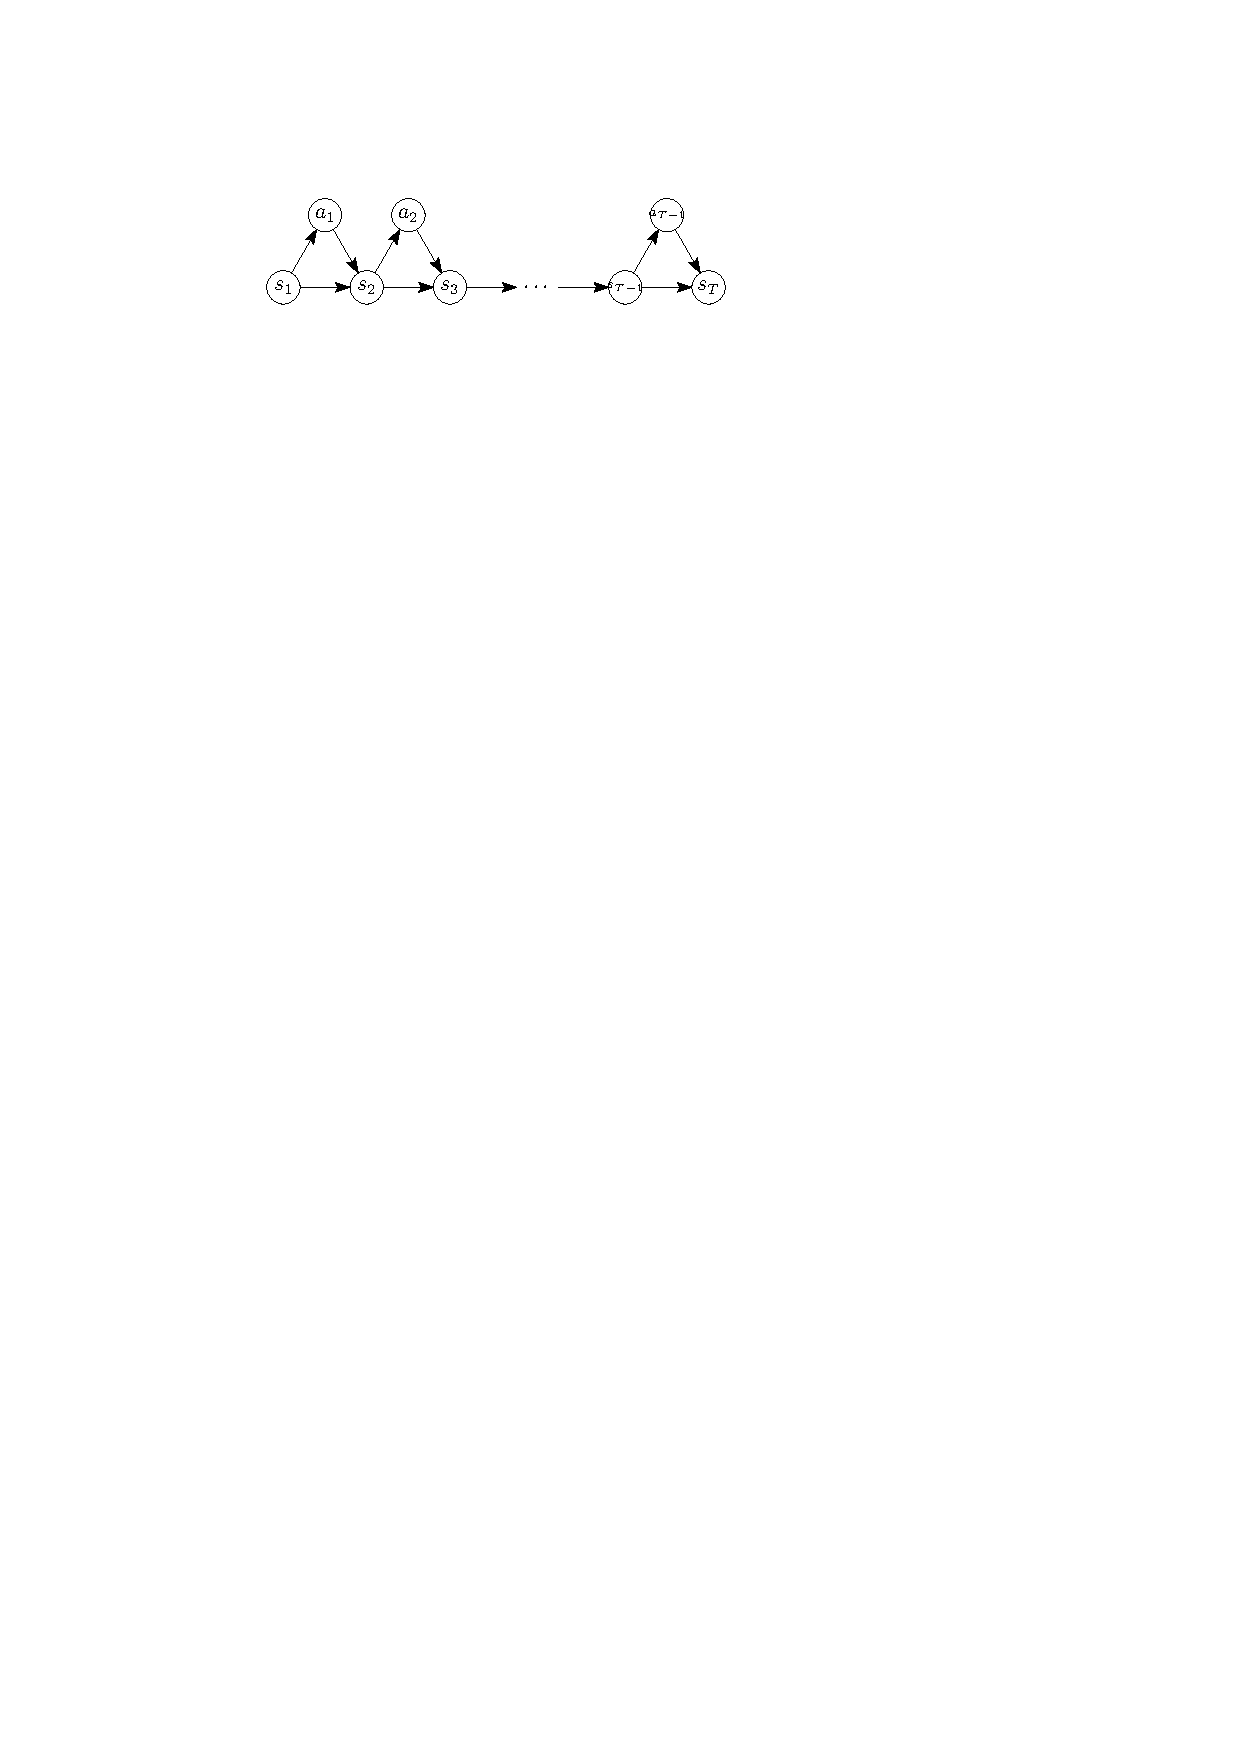
\includegraphics{image/马尔可夫决策过程.pdf}
        \end{figure}
        \[
            \begin{array}{ll}
                p(\tau) &= p(s_0,a_0,s_1,a_1,\cdots) \\
                &=p(s_0)\prod\limits_{t = 0}^{T-1}\pi(a_t|s_t)p\left( s_{t+1}|s_t,a_t \right) 
            \end{array}
        \]
        \item 给定策略$\pi\left( a|s \right)$,智能体和环境一次交互过程中的轨迹$\tau$所收到的累计奖励作为总回报
        \[
            G_t = R_{t+1}+\gamma R_{t+2}+\gamma^2R_{t+3}+\cdots
        \]
        $\gamma\in[0,1]$是折扣率。当$\gamma$接近于0时,智能体更在意短期回报;而当$\gamma$接近于1 时,长期回报变得更重要。
        \item 状态值函数:
        
        状态值函数也简称为值函数,是确定Agent 在策略$\pi$下处于某一特定状态$s$的最佳程度,即在策略$\pi$下从$s$开始获得的期望回报,表示为
        \[
            V_{\pi}(s) = E_{\pi}\left( G_t|s_t = s \right)
        \]
        根据$G_t$的表达式,可以得到
        \[
            V_{\pi}(s) = E_{\pi}\left( \sum_{k= 0}^{\infty}\gamma^kR_{t+k+1}|s_t = s \right)
        \]
        \item 状态-动作值函数(Q函数)
        
        状态-动作值函数,也称作Q 函数,用于表明遵循策略$\pi$再某一状态执行特定动作的最佳程度,也就是遵循策略$\pi$在状态$s$执行动作$a$开始获得的期望汇报
        \[
            Q^{\pi}(s,a) = E_{\pi}\left( R_{t}|s_t = s,a_t = a \right)
        \]
        根据$G_t$的表达式
        \[
            Q^{\pi}(s,a) = E_{\pi}\left(  \sum_{k= 0}^{\infty}\gamma^kR_{t+k+1}|s_t = s,a_t = a \right)
        \]
    \end{itemize}
\end{note}
\begin{example}
    强化学习只能通过马尔科夫决策过程进行建模?
    \begin{enumerate}[A]
        \item 是
        \item \textcolor{main1}{否}
    \end{enumerate}
\end{example}
\begin{note}
    最优策略与贝尔曼方程
    \begin{itemize}
        \item 强化学习的最终目的是找到一个最优策略;

        最优策略对应状态值$V$函数和$Q$函数的最大值$V^{*}(s)$和$Q^{*}(s,a)$
        \[
            \begin{array}{l}
                V^{*}(s) = \max\limits_{\pi} V^{\pi}(s)\\
                Q^{*}(s,a) = \max\limits_{\pi}Q^{\pi}(s,a)
            \end{array}
        \]
        \item 递推计算最优状态值的贝尔曼方程:
        \begin{figure}[htbp]
            \centering
            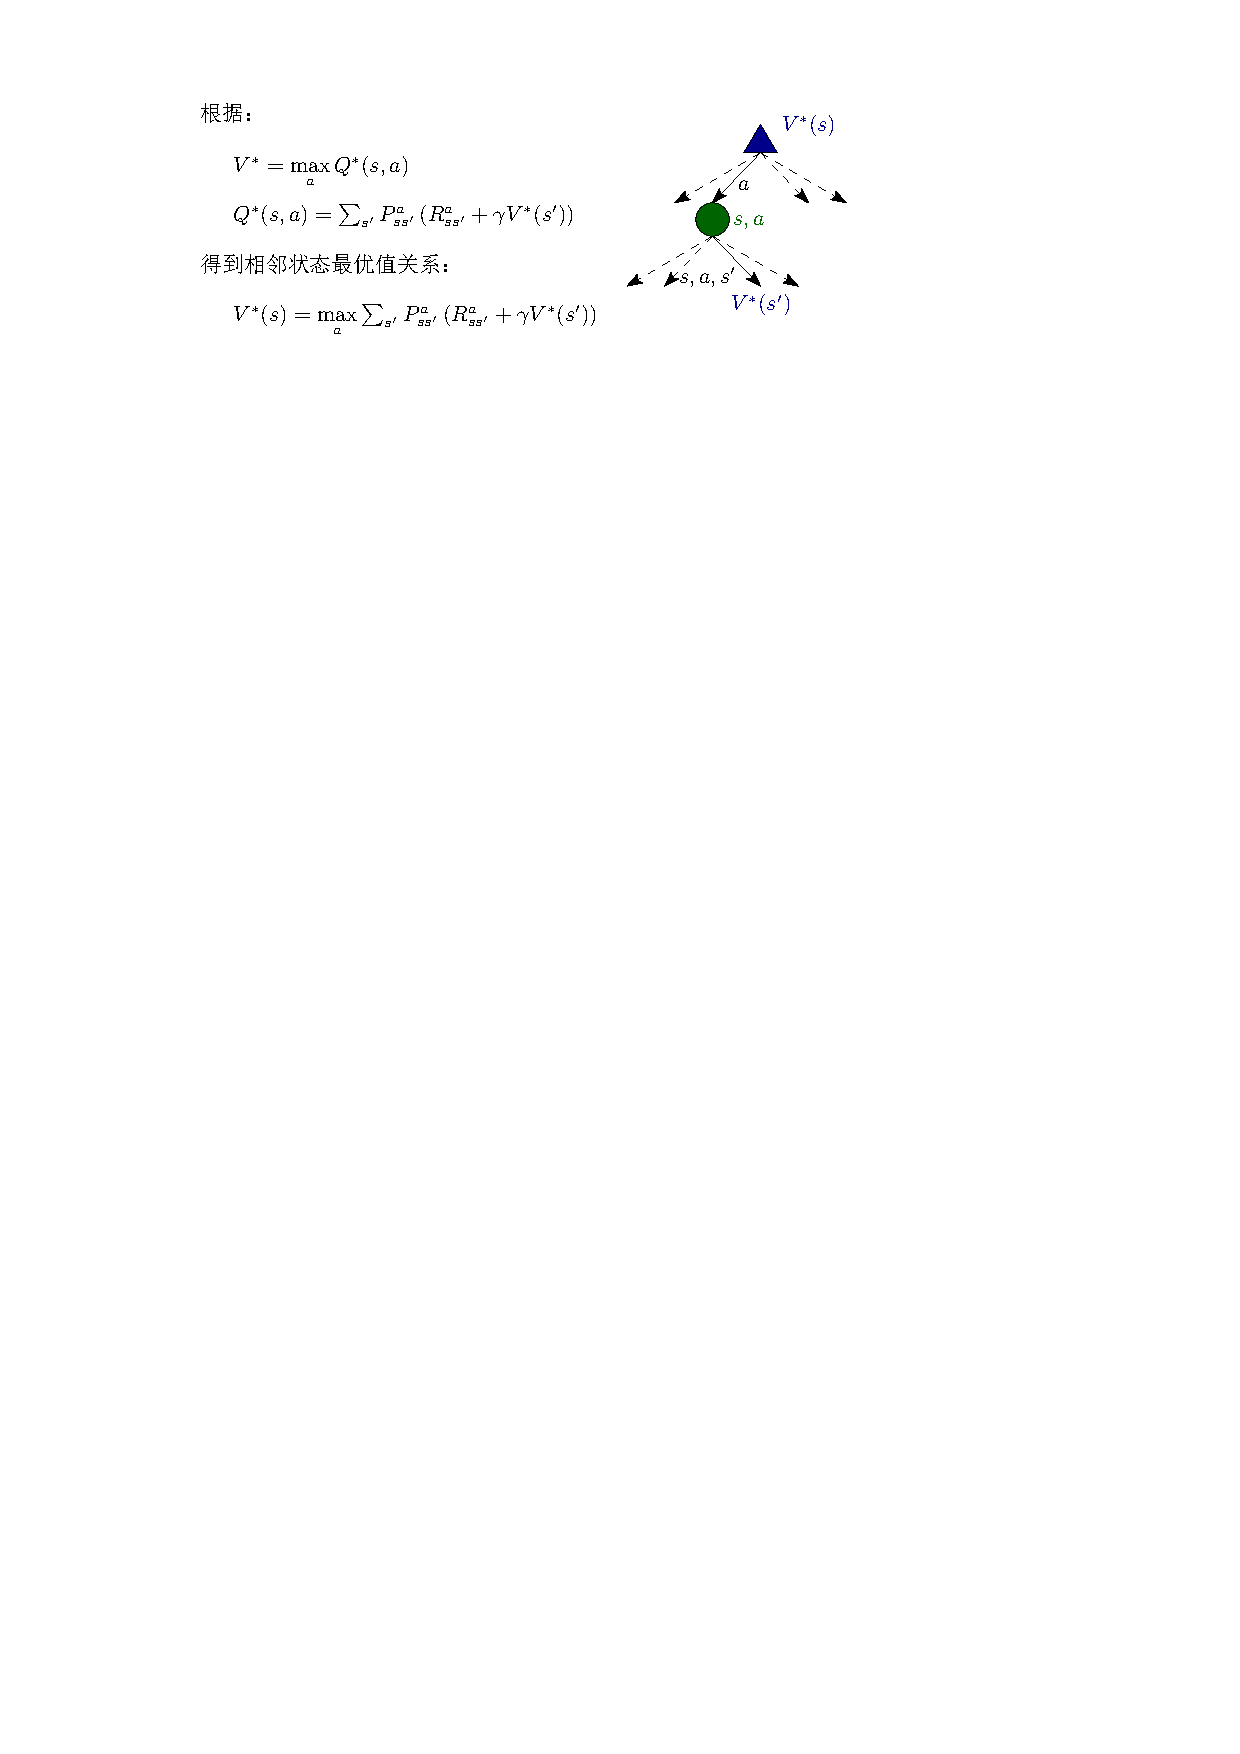
\includegraphics{image/贝尔曼方程.pdf}
        \end{figure}
        \item 可以得到对应的最优策略
        \[
            \pi^{*}(s) = \arg\max\limits_{a}\sum\limits_{s'}P_{ss'}^{a}\left( R_{ss'}^{a}+\gamma V^{*}(s') \right)
        \]
    \end{itemize}

\end{note}
\subsubsection{典型强化学习算法}
\begin{figure}[htbp]
    \centering
    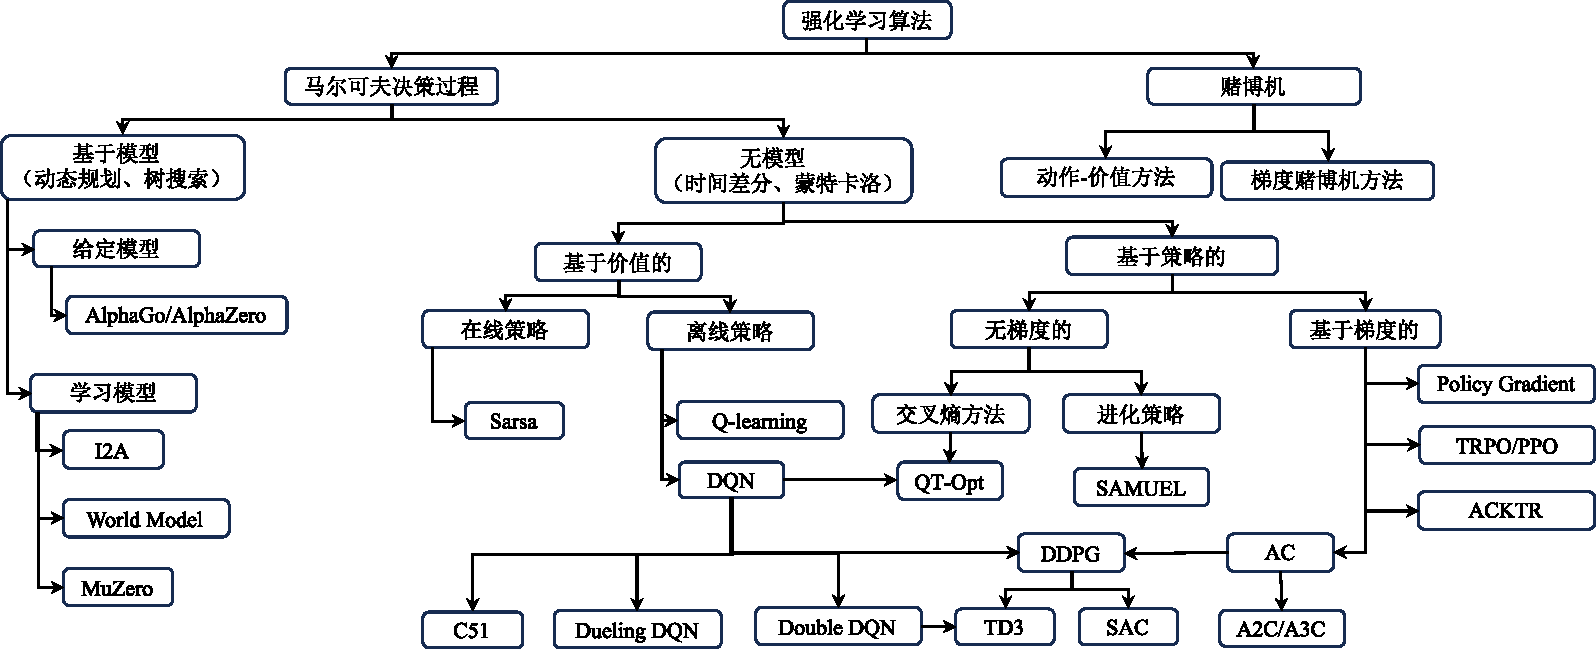
\includegraphics[width = \textwidth]{image/强化学习算法.pdf}
\end{figure}

\textcolor{red}{“模型”特指环境,即环境的动力学模型,与深度学习中的模型不同。}
\begin{figure}[htbp]
    \centering
    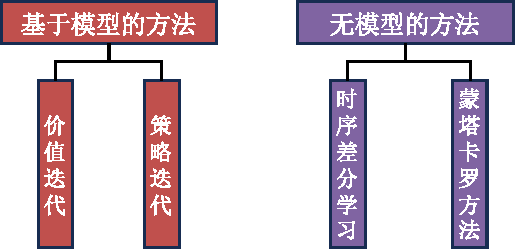
\includegraphics{image/典型强化学习算法.pdf}
\end{figure}
\begin{note}
    基于模型的方法
    \begin{itemize}
        \item 基本思想:
        \begin{itemize}
            \item 学习得到一个近似环境模型;
            \item 基于该近似模型进行求解。
        \end{itemize}
        \item 步骤一:学习训练得到模型
        \begin{itemize}
            \item 统计每个$(s,a)$情况下的结果$s'$
            \item 标准化后得到的估计值
            \item 发现$(s,a,s')$对应的奖励值
        \end{itemize}
        \item 步骤二:基于学得的模型进行求解
        \begin{itemize}
            \item 和之前一样,可以使用\textcolor{red}{价值迭代、策略迭代}等算法
        \end{itemize}
        \item 基于模型的方法:价值迭代和策略迭代均需要\textcolor{red}{环境模型(即 状态转移函数$P$和 回报函数$R$)}:
        \begin{itemize}
            \item 状态值迭代
            \[
                V_{k+1}(s) = \max\limits_{a}\sum\limits_{s'}P_{ss'}^a\left( R_{ss'}^{a}+\gamma V_{k}(s') \right),\,\forall s
            \]
            \item Q值迭代
            \[
                Q_{k+1}(s) = \arg\max\limits_{a}\sum_{s'}P_{ss'}^{a}\left( R_{ss'}^a+\gamma V_k(s') \right),\,\forall s,a
            \]
            \item 策略提炼
            \[
                \pi_{V}(s) = \arg\max\limits_{a}\sum_{s'}P_{ss'}^a\left( R_{ss'}^a+\gamma V_k(s') \right),\,\forall s
            \]
            \item 策略评估
            \[
                V_{k+1}^{\pi_i}(s) = \sum\limits_{s'}P_{ss'}^{\pi_i(s)}\left( R_{ss'}^{\pi_i(s)}+\gamma V_{k}^{\pi_i}(s') \right),\,\forall s
            \]
            \item 策略改进
            \[
                \pi_{i+1}(s) = \arg\max\limits_{a}\sum\limits_{s'}P_{ss'}\left( R_{ss'}^a+\gamma V^{\pi_{i}}(s') \right),\,\forall s
            \]
        \end{itemize}
    \end{itemize}
\end{note}
\begin{example}
    如何得到智能体的环境模型(即 P 函数和 R 函数)?
    
    规则:从A 出去减10 分,从D 出去加10 分
    \begin{figure}[htbp]
        \centering
        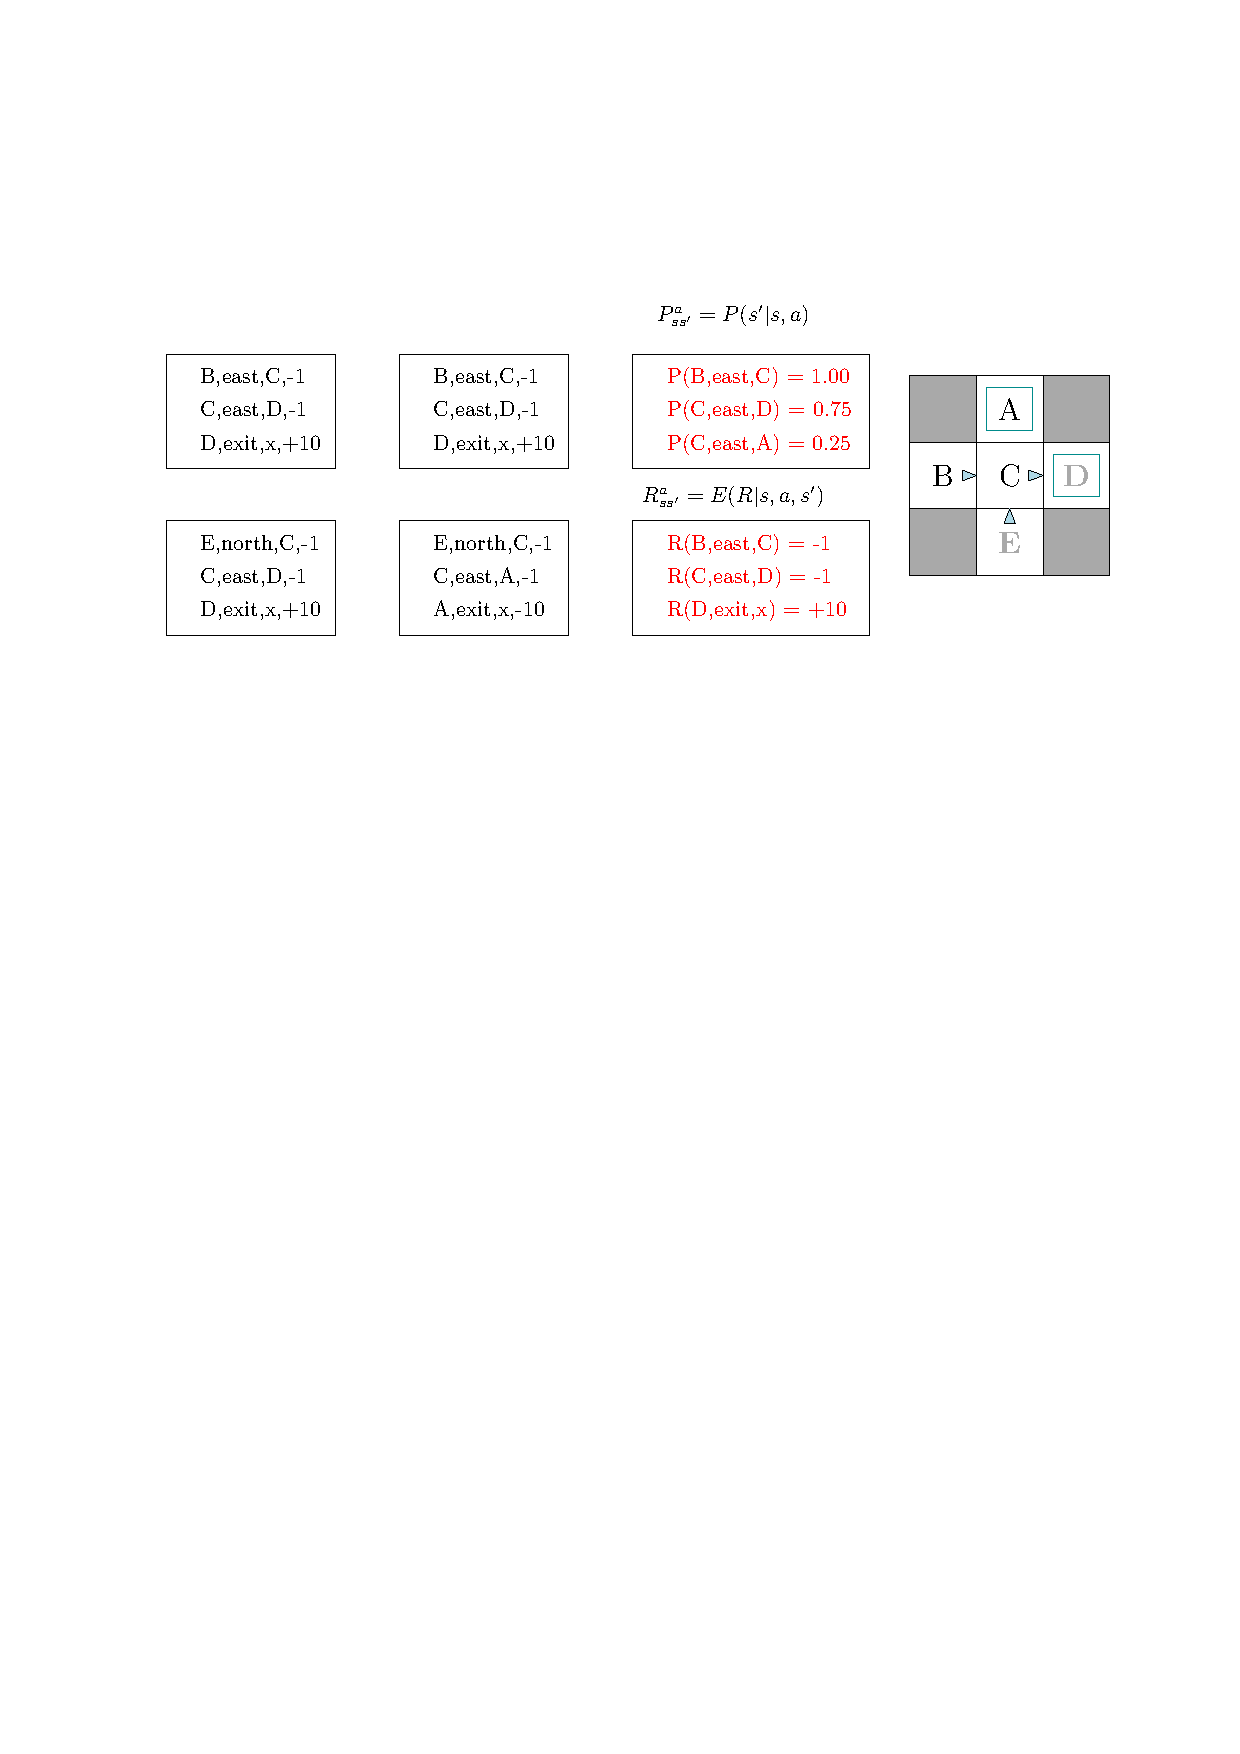
\includegraphics[width = \textwidth]{image/基于模型的方法.pdf}
    \end{figure}
\end{example}
\begin{example}
    基于模型的强化学习方法需要知道环境模型,其主要的求解方法有以下哪些?
    \begin{enumerate}[A]
        \item \textcolor{main1}{价值迭代方法}
        \item 时序差分方法
        \item \textcolor{main1}{策略迭代方法}
        \item 蒙特卡罗方法
    \end{enumerate}
\end{example}
\begin{note}
    无模型的方法\textcolor{blue}{解决$P$函数和$R$函数未知时的决策问题:}
    \begin{itemize}
        \item 状态值迭代
        \[
            V_{k+1}(s) = \max\limits_{a}\sum\limits_{s'}\cancel{P_{ss'}^a}\left( \cancel{R_{ss'}^{a}}+\gamma V_{k}(s') \right),\,\forall s
        \]
        \item Q值迭代
        \[
            Q_{k+1}(s) = \arg\max\limits_{a}\sum_{s'}\cancel{P_{ss'}^{a}}\left( \cancel{R_{ss'}^a}+\gamma V_k(s') \right),\,\forall s,a
        \]
        \item 策略提炼
        \[
            \pi_{V}(s) = \arg\max\limits_{a}\sum_{s'}\cancel{P_{ss'}^a}\left( \cancel{R_{ss'}^a}+\gamma V_k(s') \right),\,\forall s
        \]
        \item 策略评估
        \[
            V_{k+1}^{\pi_i}(s) = \sum\limits_{s'}\cancel{P_{ss'}^{\pi_i(s)}}\left( \cancel{R_{ss'}^{\pi_i(s)}}+\gamma V_{k}^{\pi_i}(s') \right),\,\forall s
        \]
        \item 策略改进
        \[
            \pi_{i+1}(s) = \arg\max\limits_{a}\sum\limits_{s'}\cancel{P_{ss'}^a}\left( \cancel{R_{ss'}^a}+\gamma V^{\pi_{i}}(s') \right),\,\forall s
        \]
    \end{itemize}
    \begin{itemize}
        \item 基本思想
        \begin{itemize}
            \item 不需要得到环境模型($P$函数和$R$函数)
            \item 直接根据环境的反馈进行学习
        \end{itemize}
        \item 典型算法:
        \begin{itemize}
            \item 时序差分学习:时序差分值学习、Q学习、Sarsa 等
            \item 蒙特卡洛方法
        \end{itemize}
    \end{itemize}
\end{note}
\begin{note}
    时序差分值学习
    \begin{itemize}
        \item 主要思想
        \begin{itemize}
            \item 基于状态转移经验$(s,a,s',r)$更新$V(s)$
            \[
                V^{\pi}(s)\gets V^{\pi}(s)+\alpha\left(r+ \gamma V^{\pi}(s')-V^{\pi}(s) \right)
            \]
            \begin{figure}[htbp]
                \centering
                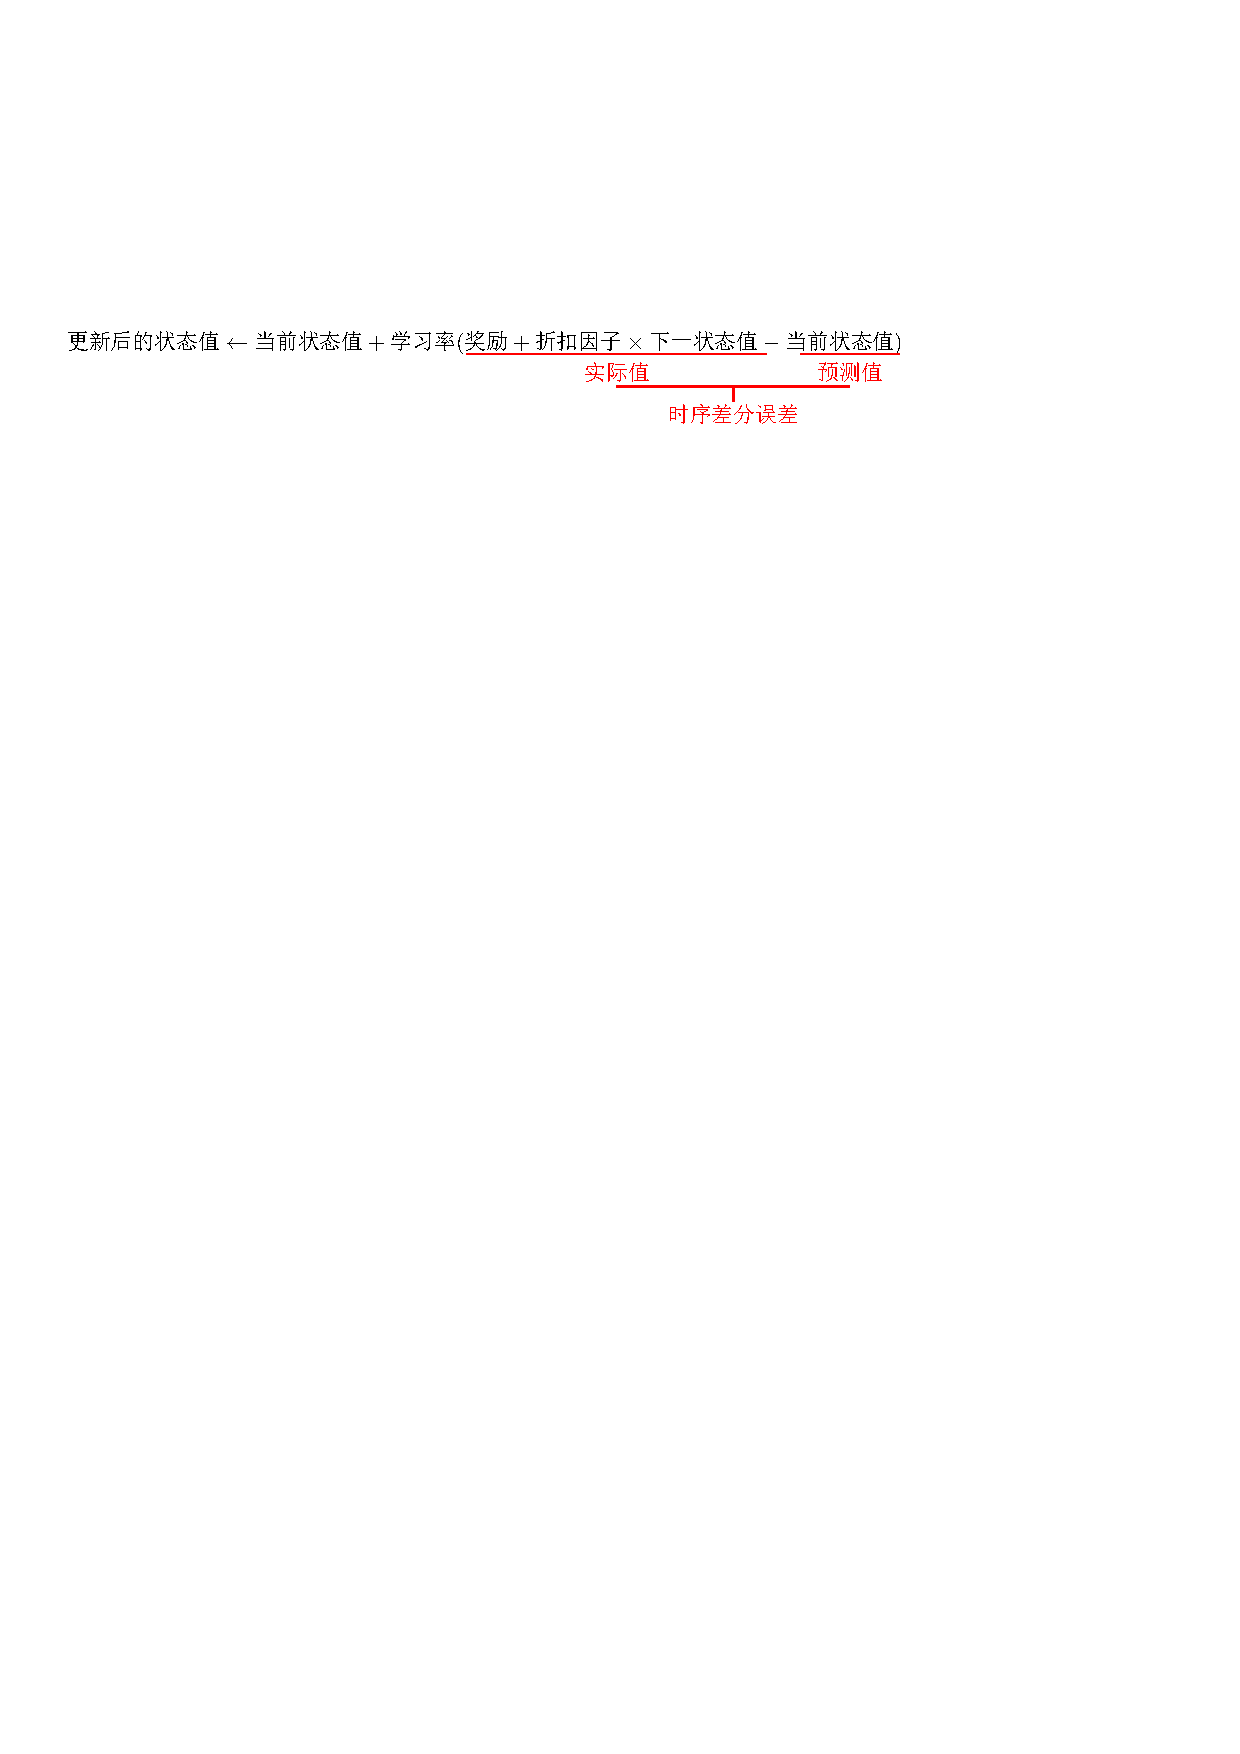
\includegraphics[width = .9\textwidth]{image/时序差分值学习思想.pdf}
            \end{figure}
            \item 实际值与预测值之差成为时序差分误差
            \item 学习率$\alpha$越大,表示采用新结果比例越大
        \end{itemize}
        \item 存在问题
        \begin{itemize}
            \item 只能估计值函数,无法对策略进行优化
        \end{itemize}
    \end{itemize}
\end{note}
\begin{example}
    举例:
    \begin{figure}[H]
        \centering
        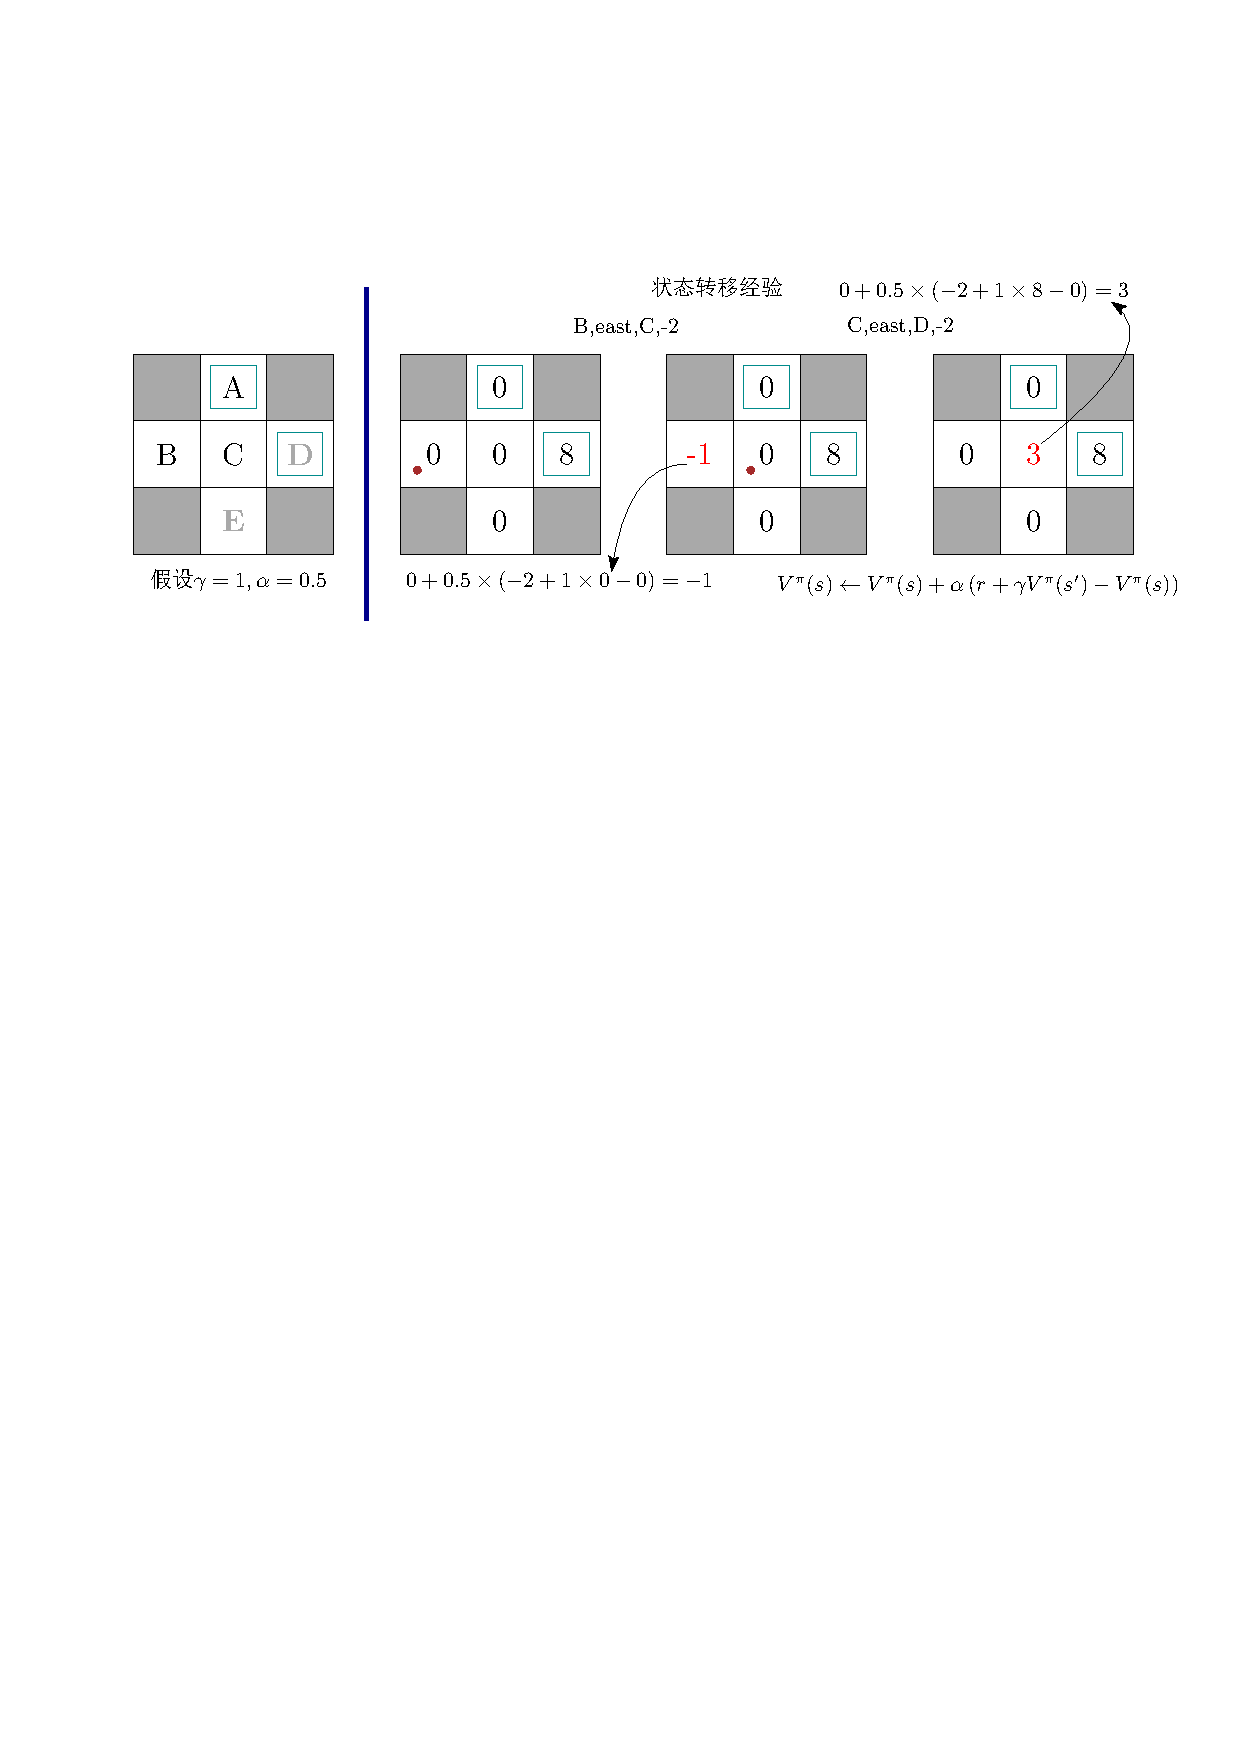
\includegraphics[width = .8\textwidth]{image/时序差分学习.pdf}
    \end{figure}
\end{example}
\begin{note}
    Q学习
    \begin{itemize}
        \item 主要思想
        \begin{itemize}
            \item 基于状态转移经验$(s,a,s',r)$更新$Q(s,a)$
            \[
                Q(s,a)\gets Q(s,a)+\alpha\left[ r+\gamma \max\limits_{\alpha'}Q(s',a')-Q(s,a) \right]
            \]
        \end{itemize}
        \item 算法流程
        \begin{figure}[htbp]
            \centering
            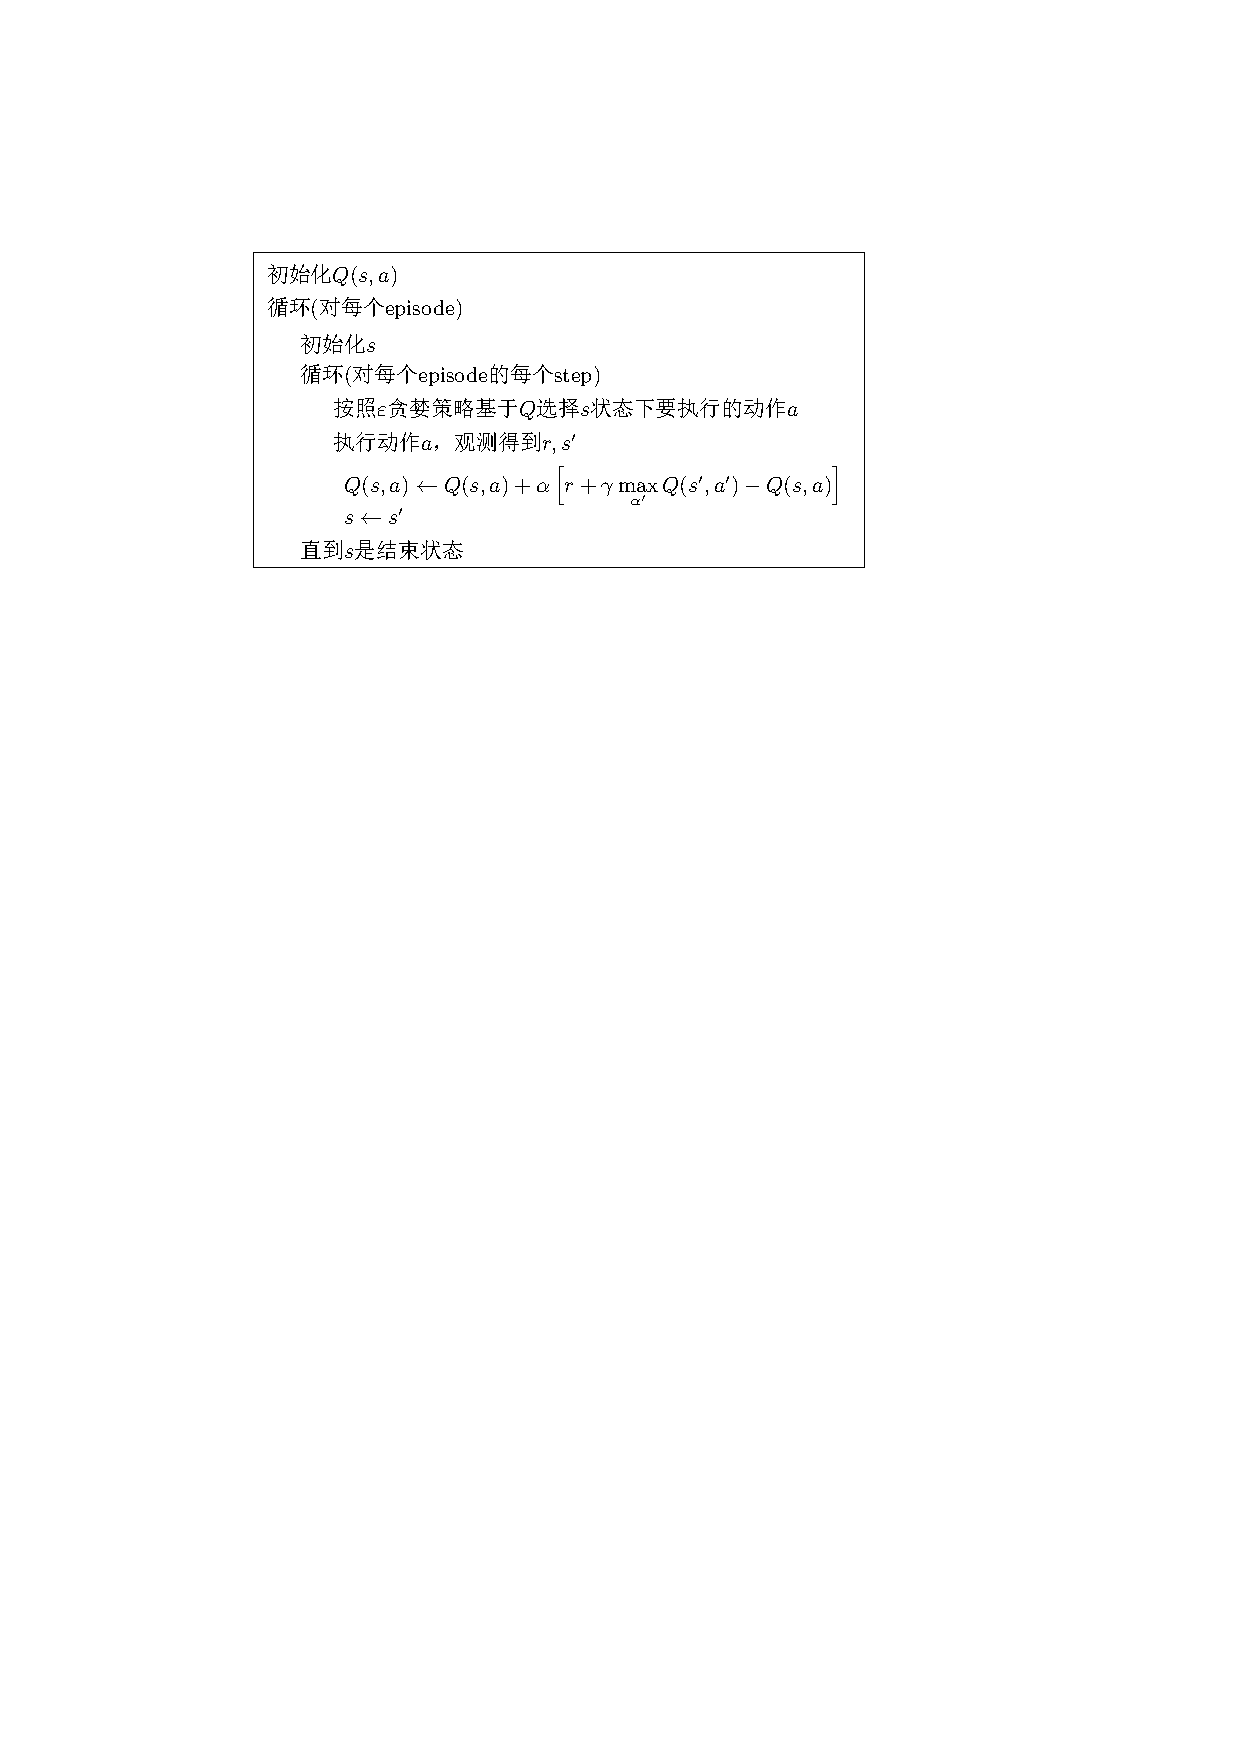
\includegraphics{image/Q学习思想.pdf}
        \end{figure}
        当满足以下两个条件是,Q学习算法能在时间趋于无穷时得到最优策略
        (1)
        \[
            \sum\limits_{t = 0}^{\infty}\alpha_{t}^2< \infty,\,\sum\limits_{t = 0}^{\infty}\alpha_{t}< \infty 
        \]

        (2)所有的状态和动作都能够被无限次遍历。
    \end{itemize}
\end{note}
\begin{example}
    Q 学习:Q学习将State 与Action 构建成一张Q-table 来存储Q 值,然后根据Q 值来选取能够获得最大的收益的动作。
    \begin{figure}[htbp]
        \centering
        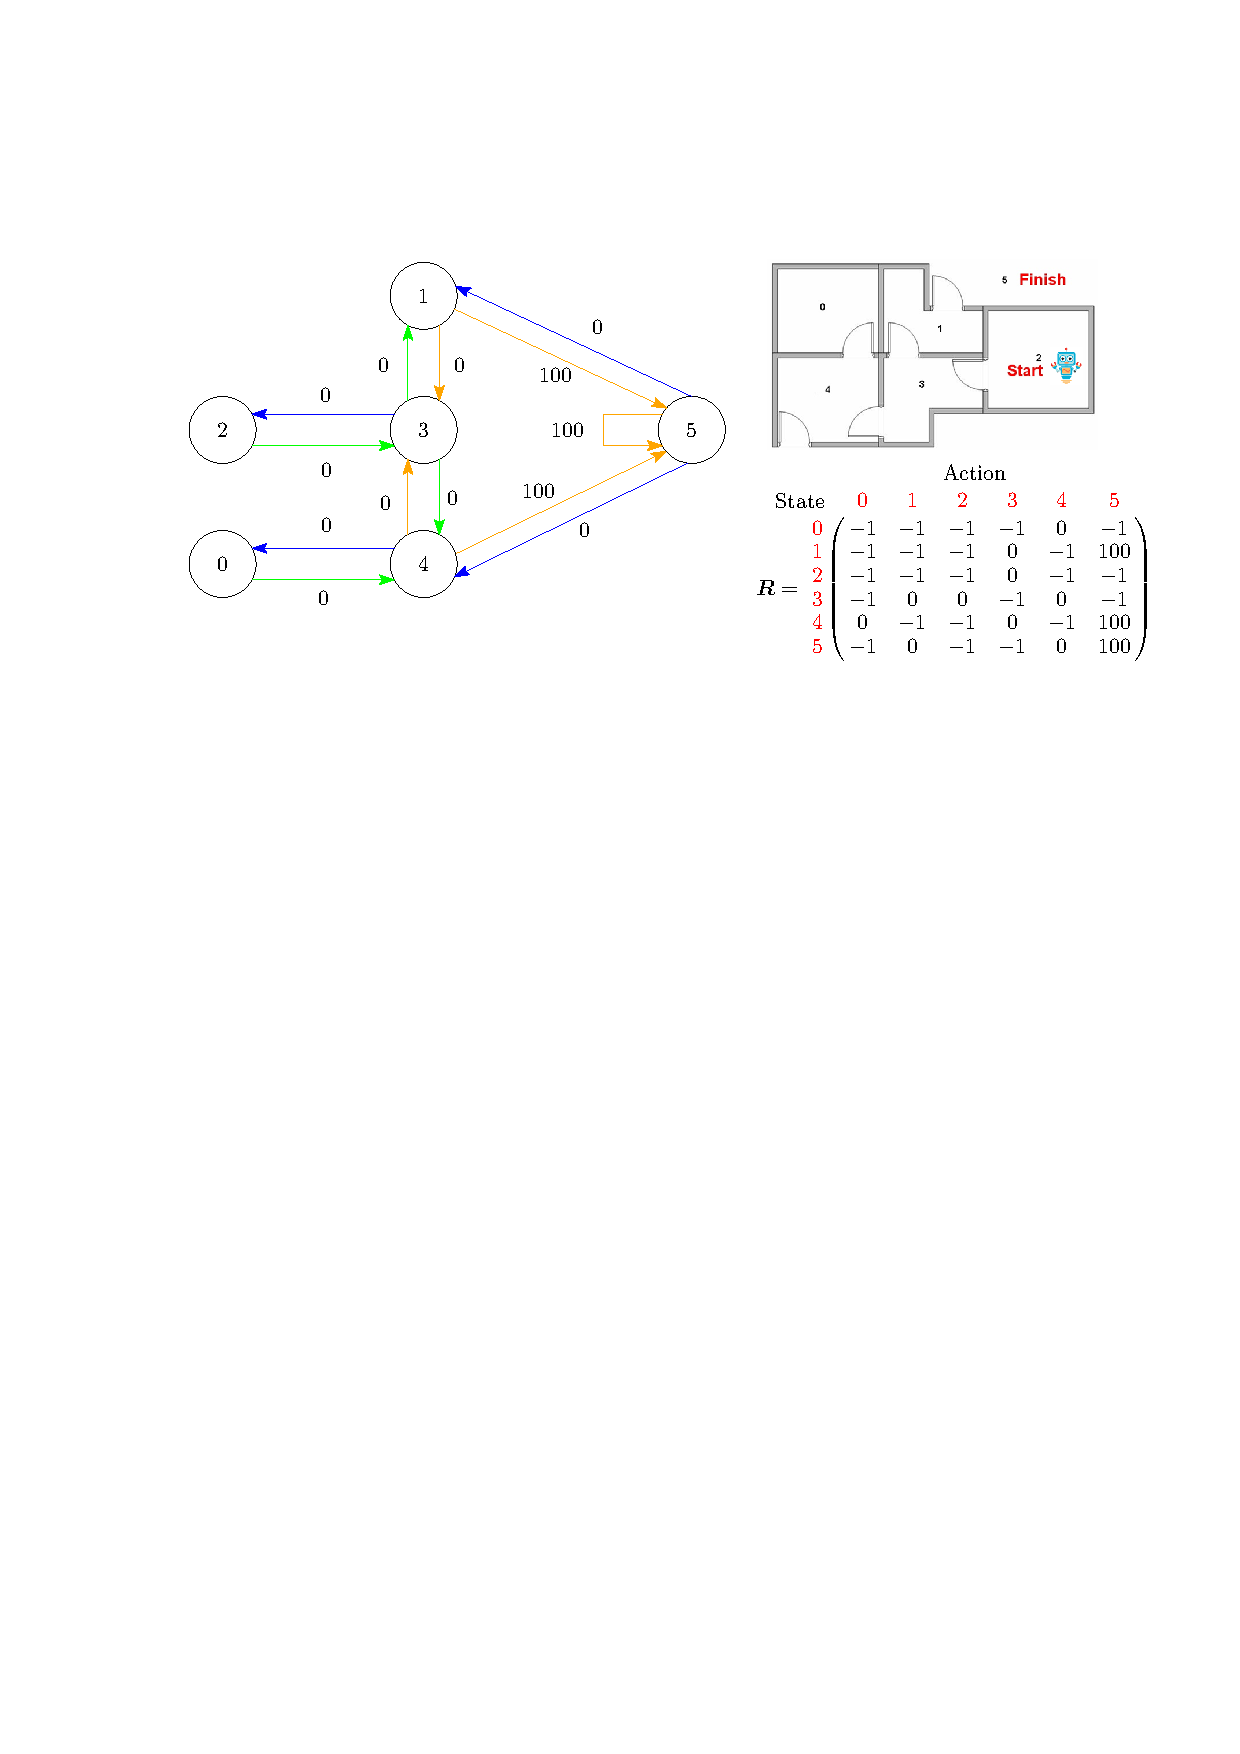
\includegraphics[scale = 0.8]{image/Q学习.pdf}
    \end{figure}
    \begin{itemize}
        \item -1表示状态之间是不互通
        \item 0表示状态之间互通,奖励为0
        \item 100表示状态之间互通,奖励为100
    \end{itemize}
    \[
        \boldsymbol{Q} =
        \bordermatrix{
            & \textcolor{red}{0} & \textcolor{red}{1} & \textcolor{red}{2} & \textcolor{red}{3} & \textcolor{red}{4} & \textcolor{red}{5} \cr
        \textcolor{red}{0} & 0   & 0   & 0   & 0   & 0   & 0 \cr
        \textcolor{red}{1} & 0   & 0   & 0   & 0   & 0   & 0 \cr
        \textcolor{red}{2} & 0   & 0   & 0   & 0   & 0   & 0 \cr
        \textcolor{red}{3} & 0   & 0   & 0   & 0   & 0   & 0 \cr
        \textcolor{red}{4} & 0   & 0   & 0   & 0   & 0   & 0 \cr
        \textcolor{red}{5} & 0   & 0   & 0   & 0   & 0   & 0 \cr
        }
    \]
    设$\gamma = 0.8,\,\alpha = 1$
    \begin{itemize}
        \item 第一局:随机性初始状态1
        \begin{itemize}
            \item 第一步:在R-table的状态1下一跳能到达状态3、5
            \item 第二步:随机选择下一跳,假设为状态5;
            \item 计算Q-table,更新,因为5是目标状态,所以完成了一轮
        \end{itemize}
        \[
            Q(1,5) = 0+1\times \left( R(1,5)+0.8\times \max\{Q(5,1),Q(5,4),Q(5,5)\}-0 \right) = 100
        \]
        \[
            \boldsymbol{Q} =
            \bordermatrix{
                & \textcolor{red}{0} & \textcolor{red}{1} & \textcolor{red}{2} & \textcolor{red}{3} & \textcolor{red}{4} & \textcolor{red}{5} \cr
            \textcolor{red}{0} & 0   & 0   & 0   & 0   & 0   & 0 \cr
            \textcolor{red}{1} & 0   & 0   & 0   & 0   & 0   & 100 \cr
            \textcolor{red}{2} & 0   & 0   & 0   & 0   & 0   & 0 \cr
            \textcolor{red}{3} & 0   & 0   & 0   & 0   & 0   & 0 \cr
            \textcolor{red}{4} & 0   & 0   & 0   & 0   & 0   & 0 \cr
            \textcolor{red}{5} & 0   & 0   & 0   & 0   & 0   & 0 \cr
            }
        \]
    \end{itemize}
    \item 第二局:随机选择初始状态3
    \begin{itemize}
        \item 第一步:在R-table 的状态3下一跳能到达状态1 、2 、4;
        \item 第二步:随机选择下一跳,假设为状态1;
        \item 在R-table 的状态1下一跳能到达状态3 、5;
        \item 第四步:计算Q-table,更新
    \end{itemize}
    \[
            Q(3,1) = 0+1\times \left( R(3,1)+0.8\times \max\{Q(1,3),Q(1,5)\}-0 \right) = 80
    \]
    经过多次循环迭代,最终得到Q-table:
    \[
        \boldsymbol{Q} =
        \bordermatrix{
            & \textcolor{red}{0} & \textcolor{red}{1} & \textcolor{red}{2} & \textcolor{red}{3} & \textcolor{red}{4} & \textcolor{red}{5} \cr
            \textcolor{red}{0} & 0   & 0   & 0   & 0   & 80  & 0 \cr
            \textcolor{red}{1} & 0   & 0   & 0   & 64  & 0   & 100 \cr
            \textcolor{red}{2} & 0   & 0   & 0   & 64  & 0   & 0 \cr
            \textcolor{red}{3} & 0   & 80  & 51  & 0   & 80  & 0 \cr
            \textcolor{red}{4} & 64  & 0   & 0   & 64  & 0   & 100 \cr
            \textcolor{red}{5} & 0   & 80  & 0   & 0   & 80  & 100 \cr
        }
    \]
    从状态2开始,智能体使用矩阵Q 计算动作
    \begin{figure}[htbp]
        \centering
        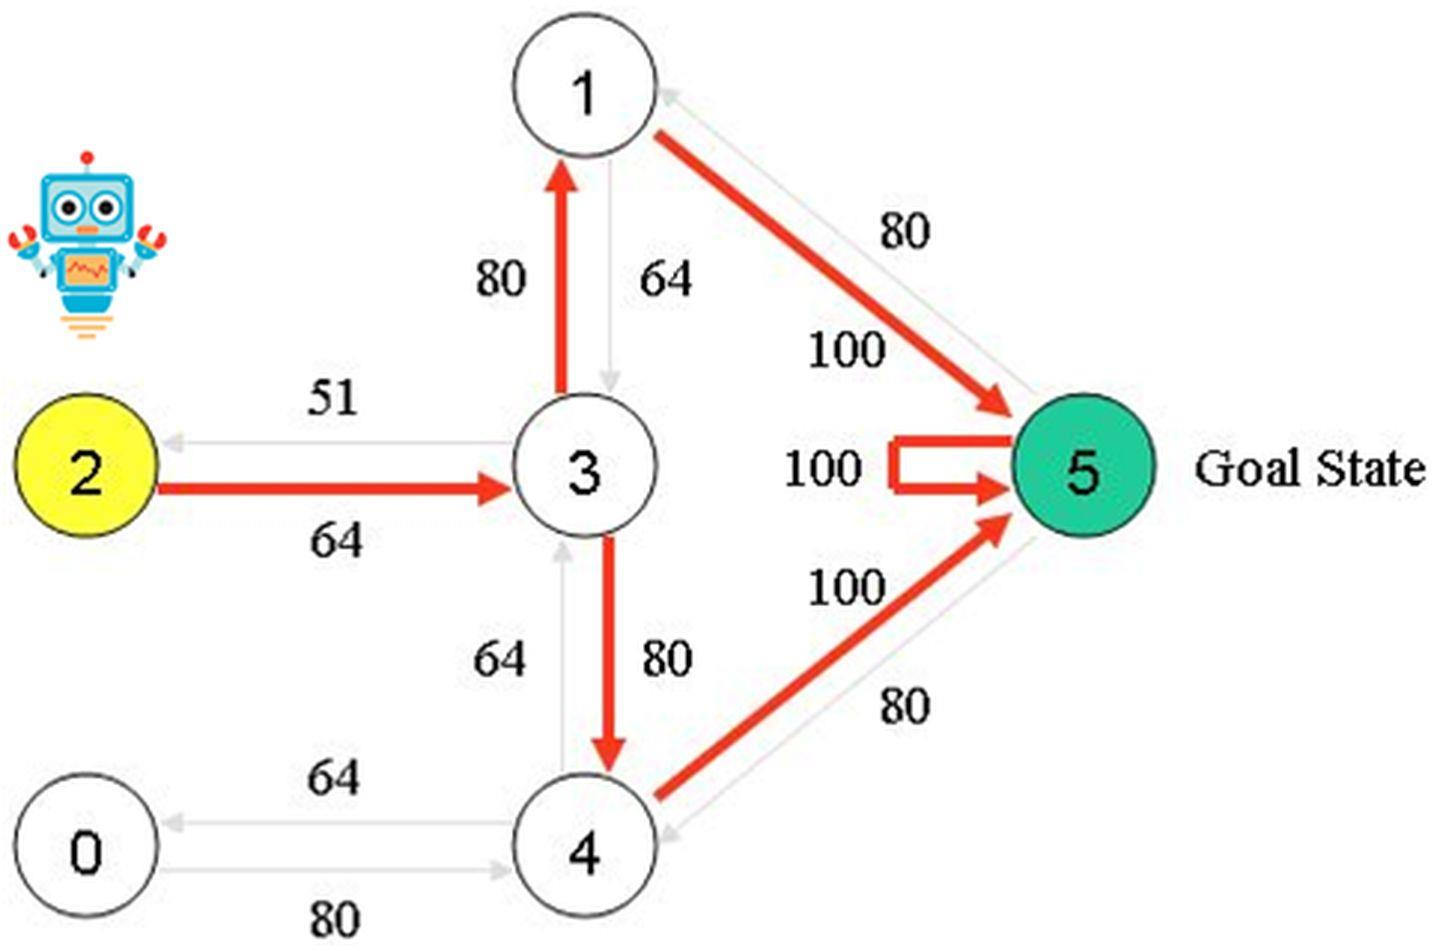
\includegraphics[width = .5\textwidth]{image/Q学习.jpg}
    \end{figure}
\end{example}
\begin{note}
    大多实际问题中状态集是庞大的无法采用矩阵形式表达,比如王者荣耀和围棋的状态空间,无法得到P 和R 函数。
\end{note}
\begin{definition}[蒙特卡罗方法]
    蒙特卡洛方法是一种无模型的方法,不需要事先知道马尔可夫决策过程的状态转移概率以及奖励,通过随机采样找到近似解,采样越多、累积奖励的平均值越接近真实的值函数。

    通过与环境交互,从所采集的样本中学习,获得关于决策过程的状态、动作和奖赏的大量数据(经验),最后计算出累积奖励的平均值。
\end{definition}
\begin{note}
    从初始状态开始,采用某种策略进行采样,执行该策略T步,获得一条轨迹:
    \[
        \left\langle s_0,a_0,r_1,s_1,a_1,r_2,\cdots,s_{T-1},a_{T-1},r_{T},s_{T} \right\rangle
    \]
    对轨迹中每一个状态-动作对,记录其的累积奖励,作为一次奖励的采样值。多次执行策略得到多条轨迹后,将每个状态-动作对的累积奖励值进行平均,得到状态-动作值函数的估计。
\end{note}
\subsection{深度强化学习}
\subsubsection{深度Q学习}
\begin{note}
    Atari游戏
    \begin{itemize}
        \item 维度灾难
        
        计算机玩Atari游戏的输入为210x160像素的原始图像数据,从理论上看,图像中每一个像素都有RGB三个通道,每个通道有256种值,总的状态空间为:
        \[
            (3\times 256)^{210\times 160}
        \]
        \item 灾难性遗忘
        
        在玩视频游戏中,人工神经网络会遭遇灾难性遗忘问题。当神经网络学会玩一种新的游戏时,原来学会的游戏就会忘掉。
    \end{itemize}
\end{note}
\begin{definition}[DQN]
    DQN思想:Q 表被深度神经网络(Q 网络)取代,后者可以把环境状态映射为智能体动作(非线性逼近)
\end{definition}
\begin{note}
    深度强化学习需要解决的2个问题:
    \begin{itemize}
        \item 深度学习需要大量有标签的数据样本;而强化学习是智能体主动获取
        样本,样本量稀疏且奖励有延迟。
        \item 深度学习要求每个样本相互之间是独立同分布的;而强化学习获取的
        相邻样本相互关联性较大,并不是相互独立的。
    \end{itemize}
\end{note}
\begin{note}
    解决问题的关键技术:
    \begin{itemize}
        \item 样本池:将采集到的样本先放入样本池,然后从样本池中随机选出一条样本用于对网络的训练。这种处理打破了样本间的关联,使样本间相互独立。
        \item 固定目标值网络:计算网络目标值需用到现有的Q 值,用一个更新较慢的网络专门提供此Q 值,提高了训练的稳定性和收敛性。
    \end{itemize}
\end{note}
\begin{note}
    DQN优缺点:
    \begin{itemize}
        \item 优点
        \begin{itemize}
            \item 算法普适性较强,相同的网络可以学习不同的Atari 游戏;
            \item 采用端到端的训练方式,无需人工提取特征,采用CNN 进行特征提取;
            \item 通过不断的训练学习,使用奖励构造标签,生成大量样本用于监督学习;
            \item 通过经验回放方法来解决样本相关性及非静态分布问题,即建立一个经验池,把每次的经验都存起来,训练时随机采样一批样本训练。
        \end{itemize}
        \item 缺点
        \begin{itemize}
            \item 只适用于处理短时记忆任务,无法处理需要长时间经验的任务
            \item 网络输出是有限离散Q 值,对应离散的动作,不能处理连续值
        \end{itemize}
    \end{itemize}
\end{note}